%%%%%%%%%%%%%%%%%%%%%%% file template.tex %%%%%%%%%%%%%%%%%%%%%%%%%
%
% This is a general template file for the LaTeX package SVJour3
% for Springer journals.          Springer Heidelberg 2010/09/16
%
% Copy it to a new file with a new name and use it as the basis
% for your article. Delete % signs as needed.
%
% This template includes a few options for different layouts and
% content for various journals. Please consult a previous issue of
% your journal as needed.
%
%%%%%%%%%%%%%%%%%%%%%%%%%%%%%%%%%%%%%%%%%%%%%%%%%%%%%%%%%%%%%%%%%%%
%
% First comes an example EPS file -- just ignore it and
% proceed on the \documentclass line
% your LaTeX will extract the file if required
\begin{filecontents*}{example.eps}
%!PS-Adobe-3.0 EPSF-3.0
%%BoundingBox: 19 19 221 221
%%CreationDate: Mon Sep 29 1997
%%Creator: programmefd by hand (JK)
%%EndComments
gsave
newpath
  20 20 moveto
  20 220 lineto
  220 220 lineto
  220 20 lineto
closepath
2 setlinewidth
gsave
  .4 setgray fill
grestore
stroke
grestore
\end{filecontents*}
%
\RequirePackage{fix-cm}
%
%\documentclass{svjour3}                     % onecolumn (standard format)
%\documentclass[smallcondensed]{svjour3}     % onecolumn (ditto)
\documentclass[smallextended]{svjour3}       % onecolumn (second format)
%\documentclass[twocolumn]{svjour3}          % twocolumn
%
\smartqed  % flush right qed marks, e.g. at end of proof

% \input{def_jiajin}

%
%\usepackage{hyperref}      % hyperlinks
\usepackage{url}            % simple URL typesetting
\usepackage{booktabs}       % professional-quality tables
\usepackage{amsfonts}       % blackboard math symbols
%\usepackage{nicefrac}       % compact symbols for 1/2, etc.
%\usepackage{microtype}      % microtypography

\usepackage{subcaption}

\usepackage{appendix}

\usepackage{mathrsfs}
\usepackage{natbib}
% Page Formatting
% \textheight 8.5in
% \addtolength{\topmargin}{-0.4in}
% \addtolength{\oddsidemargin}{-0.7in}
% \addtolength{\textwidth}{1.35in}

% for colorful table
\usepackage[table,xcdraw]{xcolor}
% for color
\definecolor{airforceblue}{rgb}{0.36, 0.54, 0.66}
\definecolor{amber}{rgb}{1.0, 0.75, 0.0}
\definecolor{burntorange}{rgb}{0.8, 0.33, 0.0}
\definecolor{dimgray}{rgb}{0.41, 0.41, 0.41}

\usepackage{hyperref} 

%\usepackage{nicematrix}
% tikz begin
\usepackage{tikz}
\usetikzlibrary{fit}
\tikzset{%
	%highlight/.style={rectangle,blend mode = multiply,fill=blue!20,fill,rounded corners = 0.3 mm,inner sep=1pt}
	highlight/.style={rectangle,blend mode = multiply,draw=blue!90!black,thick,rounded corners = 0.3 mm,inner sep=0.5pt}
}
\newcommand{\markEle}[2]{\tikz[remember picture,overlay] \node[highlight, fit = (#1-#2-medium) (#1-#2-medium)] {};}
% tikz end


\usepackage{microtype}
\usepackage{graphicx}
%\usepackage{subfigure}
\usepackage{booktabs} % for professional tables

\usepackage{amsmath,amssymb}
\usepackage[ruled,linesnumbered]{algorithm2e}
% \usepackage{algorithm,algorithmicx,algpseudocode}
% the following set font for mathbb
\usepackage{bbold}
% dsfont
\usepackage[sans]{dsfont}
% clever ref
% \usepackage[numbers]{natbib}
%\def\citep\cite
%\usepackage{natbib}
% \usepackage{cleveref}

% for circle number \ding{172} for 1
\usepackage{pifont}
% \usepackage{refcheck}
% for colors
%\usepackage{xcolor}
% for advanced theorem tools and restatable claims
\usepackage{thmtools}
\usepackage{thm-restate}

\usepackage{multirow}

% following package help make the table full textwidth
\usepackage{tabularx}

% for straight quote, use: \textquotesingle
\usepackage{textcomp}

\usepackage[shortlabels]{enumitem}
\usepackage{tikz}
\usetikzlibrary{shadows}
\usetikzlibrary{arrows,arrows.meta,positioning} 
\def\arraystretch{1.5}
\setlength\tabcolsep{2mm}
\setlength\arrayrulewidth{0.8pt}
\newcommand\hfilll{\hspace{0pt plus 1filll}}
% tikz end
%%%%%%%%%%%%%%%%%%

% for underline
% underline
\usepackage{contour}
\usepackage[normalem]{ulem}

\renewcommand{\ULdepth}{1.8pt}
\contourlength{0.8pt}

\newcommand{\myuline}[1]{%
	\uline{\phantom{#1}}%
	\llap{\contour{white}{#1}}%
}
% underline end

% equation numbering with section
\numberwithin{equation}{section}

\setlength{\tabcolsep}{3 pt}


\newcommand\Tstrut{\rule{0pt}{2.6ex}}         % = `top' strut
\newcommand\Bstrut{\rule[-0.9ex]{0pt}{0pt}}   % = `bottom' strut

% for bold greek
\usepackage{bm}

% for warp figure
\usepackage{wrapfig}
%%%%%%%%%%%% environment settings %%%%%%%%%%% 
\def \openbox{$\sqcup\llap{$\sqcap$}$}
\def \endproof{\enskip \null \nobreak \hfill \openbox \par}

\newtheorem{thm}{Theorem}
\newtheorem{ass}{Assumption}
% \newtheorem{lemma}{Lemma}
\newtheorem{prop}{Proposition}
\newtheorem{fact}{Fact}
\newtheorem{rmk}{Remark}
\newtheorem{exam}{Example}
\newtheorem{defi}{Definition}
% \newtheorem{thm}{Theorem}[subsection]
% \declaretheorem[name=Theorem,within=subsection]{thm}
% \declaretheorem[name=Lemma,sibling=thm]{lemma}
\declaretheorem[name=Corollary,sibling=thm]{coro}
\declaretheorem[name=Condition,sibling=thm]{condition}
% \declaretheorem[name=Remark,sibling=thm]{rmk}
% \declaretheorem[name=Definition,sibling=thm]{defi}
% \declaretheorem[name=Claim,sibling=thm]{claim}
% \declaretheorem[name=Conjecture,sibling=thm]{conjecture}
% \declaretheorem[name=Assumption,sibling=thm]{ass}
% \declaretheorem[name=Fact,sibling=thm]{fact}
% \declaretheorem[name=Proposition,sibling=thm]{prop}

% add comments
%\newcommand\tltodo[1]{\textcolor{blue}{[TL: #1]}}
\definecolor{amethyst}{rgb}{0.6, 0.4, 0.8}
\newcommand{\Jiajin}[1]{{\scriptsize\textbf{\color{blue}[Jiajin: #1]}}}

% \newcommand{\ceil}[1]{\left\lceil #1 \right\rceil}
% \newcommand{\floor}[1]{\left\lfloor #1 \right\rfloor}
% \newcommand{\imply}{\Rightarrow}
% \newcommand{\ifaof}{\Leftrightarrow}
% \newcommand{\limto}{\rightarrow}
% \newcommand{\del}{\partial}
% \newcommand{\bz}{\mathbf 0}
% \newcommand{\bP}{\mathbb P}
% \newcommand{\Q}{\mathbb Q}
% \newcommand{\R}{\mathbb R}
% \newcommand{\Z}{\mathbb Z}
% \newcommand{\N}{\mathbb N}
% \newcommand{\Y}{\mathbb Y}
% \newcommand{\E}[1]{{\mathbb E}\left[ #1 \right]}
% \DeclareMathOperator{\prox}{prox}
% \DeclareMathOperator{\proj}{proj}
% \DeclareMathOperator{\sign}{sign}
% \DeclareMathOperator{\res}{Res}
% \DeclareMathOperator{\dist}{dist}
% \DeclareMathOperator{\st}{s.t.}
% \DeclareMathOperator*{\argmin}{argmin}
% \DeclareMathOperator*{\argmax}{argmax}


\usepackage{tcolorbox}
\newtcbox{\alertinline}[1][red]
  {on line, arc = 0pt, outer arc = 0pt,
    colback = #1!20!white, colframe = #1!50!black,
    boxsep = 0pt, left = 1pt, right = 1pt, top = 2pt, bottom = 2pt,
    boxrule = 0pt, bottomrule = 1pt, toprule = 1pt}

% for def over equal
\newcommand{\defequal}{\overset{\text{\tiny{def}}}{=}}
\newcommand{\commentColor}{blue!90!black}

% \let\oldComment\Comment
% \renewcommand{\Comment}[1]{\oldComment{\textcolor{\commentColor}{#1}}}




\usepackage{threeparttable}
\allowdisplaybreaks[4] % spread setup 

\usepackage{tcolorbox}
%equation number 
\def\O#1{\text{\ding{\the\numexpr#1+171}}} 


%Hotkey for math notations 
\newcommand{\ceil}[1]{\left\lceil #1 \right\rceil}
\newcommand{\floor}[1]{\left\lfloor #1 \right\rfloor}
\newcommand{\imply}{\Rightarrow}
\newcommand{\ifaof}{\Leftrightarrow}
\newcommand{\limto}{\rightarrow}
\newcommand{\del}{\partial}
\newcommand{\bz}{\mathbf 0}
\newcommand{\PP}{\mathbb P}
\newcommand{\QQ}{\mathbb Q}
\newcommand{\EE}{\mathbb E}
\newcommand{\R}{\mathbb R}
\newcommand{\Z}{\mathbb Z}
\newcommand{\Y}{\mathbb Y}
%\newcommand{\E}[1]{{\mathbb E}\left[ #1 \right]}
% \newcommand{\mc}{\mathcal}
\newcommand{\diff}{\mathrm{d}}
\newcommand{\eps}{\varepsilon}
\newcommand{\Let}{\triangleq}
\DeclareMathOperator{\prox}{prox}
\DeclareMathOperator{\proj}{proj}
\DeclareMathOperator{\sign}{sign}
\DeclareMathOperator{\dist}{dist}
\DeclareMathOperator*{\argmin}{argmin}
\DeclareMathOperator*{\argmax}{argmax}


\def\A{{\mathbb{A}}}
\def\B{{\mathbb{B}}}
\def\C{{\mathbb{C}}}
\def\D{{\mathbb{D}}}
% \def\E{{\mathbb{E}}}
\def\F{{\mathbb{F}}}
\def\G{{\mathbb{G}}}
\def\H{{\mathbb{H}}}
\def\I{{\delta}}
\def\J{{\mathbb{J}}}
\def\K{{\mathbb{K}}}
\def\L{{\mathbb{L}}}
\def\M{{\mathbb{M}}}
\def\N{{\mathbb{N}}}
\def\O{{\mathbb{O}}}
\def\P{{\mathbb{P}}}
\def\Q{{\mathbb{Q}}}
\def\R{{\mathbb{R}}}
\def\S{{\mathbb{S}}}
\def\T{{\mathbb{T}}}
\def\U{{\mathbb{U}}}
\def\V{{\mathbb{V}}}
\def\W{{\mathbb{W}}}
\def\X{{\mathbb{X}}}
\def\Y{{\mathbb{Y}}}
\def\Z{{\mathbb{Z}}}

\def\bA{{\mathbf{A}}}
\def\bB{{\mathbf{B}}}
\def\bC{{\mathbf{C}}}
\def\bD{{\mathbf{D}}}
\def\bE{{\mathbf{E}}}
\def\bF{{\mathbf{F}}}
\def\bG{{\mathbf{G}}}
\def\bH{{\mathbf{H}}}
\def\bI{{\mathbf{I}}}
\def\bJ{{\mathbf{J}}}
\def\bK{{\mathbf{K}}}
\def\bL{{\mathbf{L}}}
\def\bM{{\mathbf{M}}}
\def\bN{{\mathbf{N}}}
\def\bO{{\mathbf{O}}}
\def\bP{{\mathbf{P}}}
\def\bQ{{\mathbf{Q}}}
\def\bR{{\mathbf{R}}}
\def\bS{{\mathbf{S}}}
\def\bT{{\mathbf{T}}}
\def\bU{{\mathbf{U}}}
\def\bV{{\mathbf{V}}}
\def\bW{{\mathbf{W}}}
\def\bX{{\mathbf{X}}}
\def\bY{{\mathbf{Y}}}
\def\bZ{{\mathbf{Z}}}

\def\cA{{\cal A}}
\def\cB{{\cal B}}
\def\cC{{\cal C}}
\def\cD{{\cal D}}
\def\cE{{\cal E}}
\def\cF{{\cal F}}
\def\cG{{\cal G}}
\def\cH{{\cal H}}
\def\cI{{\cal I}}
\def\cJ{{\cal J}}
\def\cK{{\cal K}}
\def\cL{{\cal L}}
\def\cM{{\cal M}}
\def\cN{{\cal N}}
\def\cO{{\cal O}}
\def\cP{{\cal P}}
\def\cQ{{\cal Q}}
\def\cR{{\cal R}}
\def\cS{{\cal S}}
\def\cT{{\cal T}}
\def\cU{{\cal U}}
\def\cV{{\cal V}}
\def\cW{{\cal W}}
\def\cX{{\cal X}}
\def\cY{{\cal Y}}
\def\cZ{{\cal Z}}

\def\a{\bm{a}}
\def\b{\bm{b}}
\def\c{\bm{c}}
\def\d{\bm{d}}
\def\e{\bm{e}}
\def\f{\bm{f}}
\def\g{\bm{g}}
\def\h{\bm{h}}
\def\i{\bm{i}}
\def\j{\bm{j}}
\def\k{\bm{k}}
\def\l{\bm{l}}
\def\m{\bm{m}}
\def\n{\bm{n}}
\def\o{\bm{o}}
\def\p{\bm{p}}
\def\q{\bm{q}}
\def\r{\bm{r}}
\def\s{\bm{s}}
\def\t{\bm{t}}
\def\u{\bm{u}}
\def\v{\bm{v}}
\def\w{\bm{w}}
\def\x{\bm{x}}
\def\y{\bm{y}}
\def\z{\bm{z}}
\def\bz{{\mathbf 0}}
\def\lbd{{\lambda}}
\def\1{{\mathbf 1}}
\def\intm{{\rm int}}
\def\bmu{\bm{\mu}}
\def\blam{\bm{\lambda}}
\def\sA{{\mathsf{A}}}
\def\sZ{{\mathsf{Z}}}

\DeclareMathOperator{\cl}{cl}
\DeclareMathOperator{\dom}{dom}
\DeclareMathOperator{\kl}{KL}
\DeclareMathOperator{\rank}{rank}
% for def over equal
% \newcommand{\defequal}{\overset{\text{\tiny{def}}}{=}}
% \newcommand{\commentColor}{blue!90!black}
%Topology related
% \DeclareMathOperator{\dim}{dim}
\DeclareMathOperator{\codim}{codim}
\DeclareMathOperator{\aff}{aff}
\DeclareMathOperator{\spann}{span}
\DeclareMathOperator{\inter}{int}
\DeclareMathOperator{\rint}{rint}
\DeclareMathOperator{\bd}{bd}
\DeclareMathOperator{\rbd}{rbd}
\DeclareMathOperator{\rand}{rand} 
% \def\keywords{\vspace{1.5em}
% {\textbf{Keywords}:\,\relax%
% }}
% \def\endkeywords{\par}

\hypersetup{colorlinks, breaklinks,
linkcolor={red!80!black},
citecolor={blue!70!black},
urlcolor={blue!70!black}}
\newcommand{\jj}[1]{{{\textbf{\color{magenta}[Jiajin: #1]}}}}


% \usepackage{mathptmx}      % use Times fonts if available on your TeX system
%
% insert here the call for the packages your document requires
%\usepackage{latexsym}
% etc.
%
% please place your own definitions here and don't use \def but
% \newcommand{}{}
%
% Insert the name of "your journal" with
% \journalname{myjournal}
%
\begin{document}

\title{\large 
Optimal  Oracle Complexity for  Weakly Convex Optimization \thanks{J. Li was supported by a Natural Sciences and Engineering Research Council of Canada
Discovery Grant RGPIN-2025-05817. }
}








% \setcounter{page}{0}



\titlerunning{
Optimal  Oracle Complexity for  Weakly Convex Optimization
}        % if too long for running head

\author{Jiajin Li   \and
        Siyu Pan
}

%\authorrunning{Short form of author list} % if too long for running head

\institute{Jiajin Li  \at
             Sauder School of Business\\ University of British Columbia, Vancouver, BC, Canada\\
              \email{jiajin.li@sauder.ubc.ca}           %  \\
%             \emph{Present address:} of \bar f. Author  %  if needed
           \and
         Siyu Pan  \at
             Sauder School of Business\\ University of British Columbia, Vancouver, BC, Canada\\
              \email{siyu.pan@sauder.ubc.ca} 
}

\date{Received: date / Accepted: date}
% The correct dates will be entered by the editor


\maketitle





\begin{abstract}
We study the oracle complexity of finding $\epsilon$-stationary
points of $\rho$-weakly convex and $G$-Lipschitz functions,
where stationarity is measured by the gradient of the Moreau
envelope. We consider an exact first-order oracle that returns both
the function value and the full subdifferential at every
query point. In the principal parameter regime, we prove that every
first-order algorithm, including randomized algorithms,
requires $\Omega(\tfrac{\rho G^2\Delta}{\epsilon^4})$ oracle queries
to succeed with any fixed positive probability, where
$f(\bz)-\inf f\le\Delta$. This lower bound matches the best known deterministic
and stochastic first-order upper bounds, up to universal
constants, and establishes the optimal randomized
first-order oracle complexity. The result separates smooth nonconvex and  weakly
convex optimization: the additional $\epsilon^{-2}$ factor
is intrinsic to nonsmooth geometry rather than stochastic
oracle noise.


\keywords{Weakly convex optimization; complexity lower bounds; oracle complexity }

\subclass{68Q25, 90C60, 49J52.}  

\end{abstract}

\section{Introduction} 
\label{sec:introduction}
The oracle complexity of finding stationary points in nonconvex
optimization is well understood in the smooth setting.
Deterministic first-order methods achieve the optimal complexity
$\Theta(\epsilon^{-2})$ \citep{CarmonEtAl2021,carmon2020lower},
whereas stochastic first-order methods require
$\Theta(\epsilon^{-4})$ oracle queries
\citep{arjevani2023lower,ghadimi2013stochastic}.

The current complexity picture for weakly convex optimization is less conclusive. Weakly convex functions encompass smooth nonconvex and convex-composite objectives
\citep{vial1983strong,drusvyatskiy2019efficiency}, and provide a broad setting for nonsmooth nonconvex optimization.
For this class, stochastic subgradient methods achieve an oracle
complexity of $\mathcal O(\epsilon^{-4})$ for finding an
$\epsilon$-stationary point, where stationarity is measured by
the gradient of the Moreau envelope
\citep{DavisDrusvyatskiy2019,davis2019proximally,davis2018stochastic}.
This naturally raises the following question:
\begin{center}
    \bf Can deterministic first-order methods break the $\epsilon^{-4}$ barrier?
\end{center}
We show that the $\epsilon^{-4}$ dependence is already necessary
for deterministic first-order methods.
Moreover, allowing algorithms to randomize their queries does
not improve this dependence even with exact first-order oracles.
This reveals a fundamental distinction between smooth nonconvex
and  weakly convex optimization: the additional
$\epsilon^{-2}$ factor is intrinsic to nonsmooth geometry. This separation parallels the classical gap between smooth and
nonsmooth convex optimization
\citep{nesterov2013introductory,bubeck2015convex},
but concerns stationarity rather than objective suboptimality. 

Specifically, we study the oracle complexity of the weakly convex
optimization problem
\begin{equation}
\label{eq:prob}
\min_{\x\in\mathbb R^d} f(\x),
\tag{P}
\end{equation} 
where \(f:\mathbb R^d\to\mathbb R\) is globally \(G\)-Lipschitz,
\(\rho\)-weakly convex for some \(\rho>0\), and possibly nonsmooth. We assume that \(f(\bz)-\inf f\le\Delta\).
Let \(f_\lambda\) denote the Moreau envelope of \(f\), with
\(\lambda=\tfrac{1}{2\rho}\).
For \(\epsilon>0\), we call a point \(\x\in\mathbb R^d\)
\(\epsilon\)-stationary if
$
\|\nabla f_\lambda(\x)\|\le\epsilon.
$ 
We adopt a first-order oracle that returns both the function value
and the \emph{full subdifferential} at every query point.
This stronger oracle ensures that our lower bound does not rely
on an unfavorable choice of subgradient by the oracle. 

\subsection{Our results and techniques} 
We first state an informal version of our main lower bound
\begin{theorem}[Informal]
In the principal parameter regime, the randomized first-order
oracle complexity of finding an \(\epsilon\)-stationary point
with probability at least \(1-\nu\) is
\[
\Omega\!\left(\frac{\rho G^2\Delta}{\epsilon^4}\right),
\]
with universal implied constants for every \(\nu\in(0,1)\).
\end{theorem}
To prove this result, we generalize the classical
zero-chain construction
\citep{nesterov2013introductory,CarmonEtAl2021}
in two directions.
First, we extend the zero-chain property to the full
subdifferential oracle. We construct a tilted max-affine
convex block $\phi:\R^N\to\R$ whose entire subdifferential
satisfies the following \emph{setwise zero-chain property} for every $n\in\{0,\ldots,N-1\}$: 
\[
 \x\in\operatorname{span}\{\mathbf e_1,\ldots,\mathbf e_n\}
 \quad\Longrightarrow\quad
 \partial \phi(\x)\subseteq
 \operatorname{span}\{\mathbf e_1,\ldots,\mathbf e_{n+1}\}.
\]
Thus even observing the entire subdifferential reveals
at most one new coordinate. 

Second, we couple $M$ setwise zero-chain blocks
to construct a weakly convex hard instance.
The coupling permits simultaneous activation of
neighboring blocks, so the classical coordinatewise
zero-chain property is no longer preserved.
To track this simultaneous progress, we organize
coordinates across blocks into diagonal layers,
each containing at most a universal constant
number of coordinate directions.
We establish a generalized zero-chain property
with respect to the resulting filtration,
yielding an oracle horizon of order $MN$; see
Figure~\ref{fig:overlapping-relay}.
In the stated parameter regime, we take
$N=\Theta(\tfrac{G^2}{\epsilon^2})$ and
$M=\Theta(\tfrac{\rho\Delta}{\epsilon^2})$, giving
$MN=\Theta(\tfrac{\rho G^2\Delta}{\epsilon^4})$.
% Latest version: blocks 1, 2, 3, ..., M.

\usetikzlibrary{arrows.meta}
\begin{figure}[t]
\centering
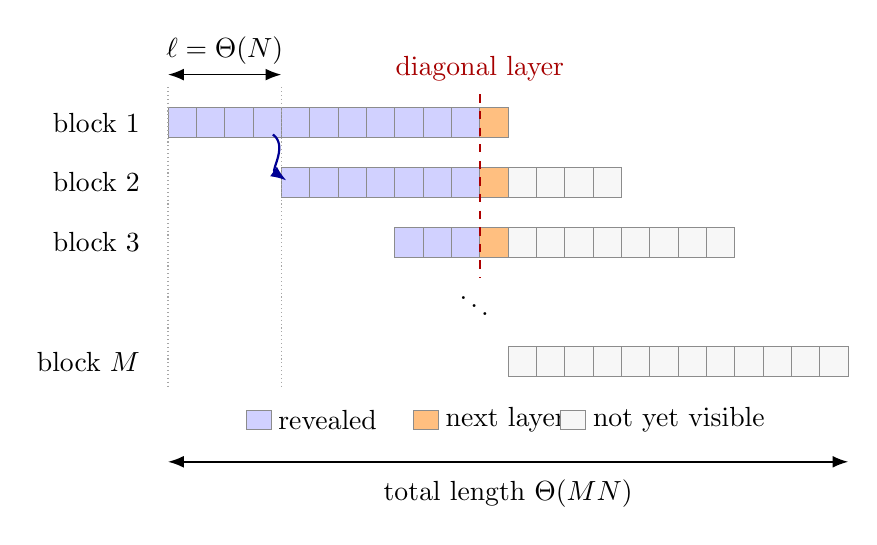
\begin{tikzpicture}[
    x=0.36cm,
    y=0.76cm,
    cell/.style={
      draw=black!45,
      line width=0.35pt,
      minimum width=0.36cm,
      minimum height=0.38cm,
      inner sep=0pt
    },
    revealed/.style={cell,fill=blue!18},
    frontier/.style={cell,fill=orange!50},
    hidden/.style={cell,fill=black!3},
    >=Latex
]
\def\BlockLength{12}
\def\RelayDelay{4}
\def\CurrentLevel{10}
\def\TotalDepth{24}

% The first three blocks.
\pgfmathtruncatemacro{\NextLevel}{\CurrentLevel+1}
\foreach \m in {1,2,3} {
  \pgfmathtruncatemacro{\shift}{(\m-1)*\RelayDelay}
  \pgfmathtruncatemacro{\yy}{1-\m}

  \node[anchor=east]
    at (-0.65,\yy+0.25) {block \(\m\)};

  \foreach \j in {1,...,\BlockLength} {
    \pgfmathtruncatemacro{\lev}{\shift+\j-1}
    \ifnum\lev<\NextLevel
      \node[revealed] at (\lev+0.5,\yy+0.25) {};
    \else
      \ifnum\lev=\NextLevel
        \node[frontier] at (\lev+0.5,\yy+0.25) {};
      \else
        \node[hidden] at (\lev+0.5,\yy+0.25) {};
      \fi
    \fi
  }
}

% Omitted intermediate blocks and the terminal block.
\node at (10.8,-2.68) {\(\ddots\)};
\node[anchor=east] at (-0.65,-3.75) {block \(M\)};

\foreach \j in {1,...,\BlockLength} {
  \pgfmathtruncatemacro{\xx}{12+\j-1}
  \node[hidden] at (\xx+0.5,-3.75) {};
}

% Delay between consecutive block starts.
\draw[<->,line width=0.6pt]
  (0,1.05)--(\RelayDelay,1.05)
  node[midway,above] {\(\ell=\Theta(N)\)};

\draw[densely dotted,black!35]
  (0,0.84)--(0,-4.15);
\draw[densely dotted,black!35]
  (\RelayDelay,0.84)--(\RelayDelay,-4.15);

% Relay to the next block.
\draw[-{Latex[length=2mm]},blue!58!black,line width=0.8pt]
  (\RelayDelay-0.30,0.05)
  to[out=-36,in=145]
  (\RelayDelay+0.18,-0.72);

% One diagonal layer in the shifted display.
\draw[dashed,red!68!black,line width=0.75pt]
  (\NextLevel,0.72)--(\NextLevel,-2.35);
\node[anchor=south,text=red!65!black]
  at (\NextLevel,0.79) {diagonal layer};

% Legend.
\node[revealed,minimum width=0.32cm,minimum height=0.25cm]
  at (3.2,-4.72) {};
\node[anchor=west]
  at (3.55,-4.72) {revealed};

\node[frontier,minimum width=0.32cm,minimum height=0.25cm]
  at (9.1,-4.72) {};
\node[anchor=west]
  at (9.45,-4.72) {next layer};

\node[hidden,minimum width=0.32cm,minimum height=0.25cm]
  at (14.3,-4.72) {};
\node[anchor=west]
  at (14.65,-4.72) {not yet visible};

% Total length.
\draw[<->,line width=0.6pt]
  (0,-5.42)--(\TotalDepth,-5.42)
  node[midway,below=3pt] {total length \(\Theta(MN)\)};

\end{tikzpicture}
\caption{Schematic of the overlapping relay across blocks.}
\label{fig:overlapping-relay}
\end{figure}

Finally, we extend the lower bound to arbitrary randomized
first-order algorithms with the full subdifferential oracle.
We combine the radial modification of Diakonikolas and
Guzm\'an \citep[Section~2.1]{DiakonikolasGuzman2020}
with a simplified adaptation of the random-rotation
argument of Carmon et al.\
\citep[Section~5.1]{carmon2020lower}.

\paragraph{Notation.}
Bold lowercase letters denote vectors, with scalar coordinates
written without boldface. We use $\langle\cdot,\cdot\rangle$,
$\|\cdot\|$, and $\|\cdot\|_1$ for the Euclidean inner product,
Euclidean norm, and $\ell_1$ norm, respectively.
We write $\N:=\{1,2,\ldots\}$, $\N_0:=\N\cup\{0\}$,
$[n]:=\{1,\ldots,n\}$, and $[0]:=\varnothing$,
and adopt $\inf\varnothing:=+\infty$ and
$\operatorname{span}\varnothing:=\{\bz\}$.
The symbols $\bz$, $\bm e_i$ (or $\bm e_{mn}$ for block
coordinates), and $\mathbf I_d$ denote the zero vector,
standard basis vectors, and identity matrix, respectively.
Vector inequalities are componentwise; $\wedge$ and $\vee$
denote componentwise minimum and maximum, respectively.
We write $[\x]_+:=(\max\{x_i,0\})_i$ and
$\operatorname{supp}(\x):=\{i:x_i\ne0\}$.
For a set $S$, $\operatorname{conv}S$ denotes its convex hull
and $\operatorname{dist}(\x,S):=\inf_{\y\in S}\|\x-\y\|$.
Finally, $\operatorname{Lip}(g)$ denotes the  Lipschitz
constant of $g$, and $\prox_{\lambda f}(\x)$ denotes the
minimizer defining $f_\lambda(\x)$ when it is unique.

\paragraph{Structure of the paper.} Section~\ref{sec:pre} introduces the function class,
stationarity measure, and oracle model.
Section~\ref{sec:main} states the main result
and presents an abstract lower-bound framework.
Section~\ref{sec:construction} constructs the unscaled
hard instance, and Section~\ref{sec:verification}
verifies its required properties.
Section~\ref{sec:proof} completes the proof through
the radial modification, random rotation, and rescaling.



\section{Preliminaries}
\label{sec:pre}  
This section introduces the function class, stationarity
measure, and full subdifferential oracle. We then define the class of randomized first-order algorithms and the
associated oracle complexity.
\begin{definition}[Function class]
Suppose that \(G,\rho>0\) and \(\Delta\geq0\). We define \(\mathcal F(G,\rho,\Delta)\)
as the union, over dimensions \(d\in\N\), of the classes of functions
\(f:\R^d\to\R\) satisfying the following properties:
\begin{enumerate}[label=(\roman*)]
 \item (\(\rho\)-weak convexity) \(f\) is \(\rho\)-weakly convex,
 {i.e., $\x\mapsto f(\x)+\tfrac\rho2\|\x\|^2$ is convex.} 
 \item ($G$-Lipschitz continuity) $f$ is $G$-Lipschitz, i.e., for all $\x,\y\in \R^d$, 
 $$
 |f(\x)-f(\y)|\leq G\|\x-\y\|. 
 $$
 \item (Initial gap)  The initialization satisfies $f(\bz)-\inf_{\x\in\R^d} f(\x)\leq\Delta$.
\end{enumerate}
\end{definition}
We introduce the stationarity measure used throughout the paper. 
\begin{definition}[$\epsilon$-stationary point]
\label{def:stationary}
Let $\lambda = \tfrac{1}{2\rho}$, and define the Moreau envelope of $f$ by
\[
f_\lambda(\x)
:=
\min_{\z\in\R^d}
\left\{
f(\z)+\frac{1}{2\lambda}\|\x-\z\|^2
\right\}.
\]
Given $\epsilon>0$, a point $\x\in\R^d$ is an
$\epsilon$-stationary point of problem \eqref{eq:prob} if
$
\|\nabla f_\lambda(\x)\|\leq\epsilon.
$ 
\end{definition}
We consider the generalized first-order oracle (FO), denoted by
$\mathbb O_f(\x)$. For finite-valued weakly convex functions on $\R^d$, the
Fr\'echet, limiting (Mordukhovich), and Clarke subdifferentials
coincide at every point, and their common value is a nonempty
compact convex set
\citep{rockafellar2009variational,clarke1990optimization,
mordukhovich2006variational}.
We call functions in $\mathcal F(G,\rho,\Delta)$ admissible. 
\begin{definition}[{First-order oracle}]
For each query point \(\x\in\R^d\) and each admissible \(f\), the first-order oracle returns both the function value and the full subdifferential set, i.e.,
$\mathbb{O}_f(\x) := (f(\x),\partial f(\x))$. 
\end{definition}
Let $\mathcal K_d$ denote the space of nonempty compact convex
subsets of $\R^d$, equipped with the Borel $\sigma$-algebra
induced by the Hausdorff metric.

\begin{definition}[Randomized first-order algorithm]
\label{def:randomized-algorithm}
A randomized first-order algorithm $\sA$ is specified by
a private random seed
$\xi_{\sA}\sim\operatorname{Unif}[0,1]$, drawn independently
of $f$, and a sequence of Borel measurable maps
\[
\Gamma_t:
[0,1]\times(\R\times\mathcal K_d)^t
\longrightarrow \R^d,
\qquad t\geq1.
\]
An algorithm is understood as a family of such maps,
one for each dimension $d$; we suppress the dimension index.
For every admissible $f$, the algorithm starts from
$\sA^{(0)}[f]=\bz$ and generates its queries according to
\[
\sA^{(t)}[f]
=
\Gamma_t\left(
    \xi_{\sA},
    \bigl(
        \mathbb O_f(\sA^{(s)}[f])
    \bigr)_{s=0}^{t-1}
\right),
\qquad t\geq1.
\]
We denote the class of such algorithms by
$\mathcal A_{\rand}$.
\end{definition}
Notably, deterministic first-order algorithms form a subclass of
$\mathcal A_{\rand}$, obtained by choosing decision maps
$\Gamma_t$ that do not depend on the random seed $\xi_{\sA}$.
Consequently, our lower bounds for randomized algorithms
also apply to deterministic first-order algorithms.

Adapting the oracle-complexity framework of
Carmon et al.~\citep{CarmonEtAl2021} to our setting,
we introduce the complexity measure used throughout the paper. 
\begin{definition}[Oracle complexity]
\label{def:complexity-algorithm-class}
Fix a stationarity tolerance \(\epsilon>0\) and a confidence level
\(1-\nu\), where \(\nu\in[0,1)\). Let
\(\cA\subseteq\cA_{\rand}\) be any nonempty subclass of randomized
first-order algorithms, and let \(\cF\) be a nonempty admissible
function class. The oracle complexity of \(\cA\) on \(\cF\), i.e., $\cT_{\epsilon,\nu}(\cA,\cF)$, is
defined by
\[
    % \cT_{\epsilon,\nu}(\cA,\cF)
    % :=
    {\color{black}\inf_{\sA\in\cA}
    \sup_{f\in\cF}
    \inf}
    \left\{
        t\in\N_0
        \;\middle|\;
        \P_{\xi_{\sA}}
        \left(
            \sA^{(t)}[f]
            \text{ is an }\epsilon\text{-stationary point of }f
        \right)
        \geq 1-\nu
    \right\},
\]
where \(\P_{\xi_{\sA}}\) denotes probability with respect to the
internal seed \(\xi_{\sA}\) of the algorithm, as introduced in
Definition~\ref{def:randomized-algorithm}.
\end{definition}
% Here $\N_0:=\{0,1,2,\ldots\}$ and $\inf\varnothing:=+\infty$.
The output $\sA^{(t)}[f]$ is formed after $t$ oracle replies
and need not itself be queried. In particular, $t=0$
allows returning the initial point $\bz$. 
\section{Main Results and An Abstract Lower Bound Framework}
 \label{sec:main}
\subsection{Main results}
\begin{theorem}
\label{thm:main}
There exists a universal constant $c_0>0$ such that the following holds.
Let $G,\rho, \Delta>0$. Suppose that $0<\epsilon\le c_0\min\{G,\sqrt{\rho\Delta}\}$ and $\Delta\leq\tfrac{G^2}{\rho}
       \exp\left(\tfrac{G^2}{200\epsilon^2}\right)$. 
Then, for every $\nu\in[0,1)$,
\[
\mathcal T_{\epsilon,\nu}
\bigl(\mathcal A_{\rand},\mathcal F(G,\rho,\Delta)\bigr)
=
\Omega\left(\frac{\rho G^2\Delta}{\epsilon^4}\right),
\]
with universal  constants independent of $\nu$. 
\end{theorem}
The lower bound allows any output that is a Borel measurable
function of the algorithm's private seed and oracle transcript;
the output need not itself be queried.
Moreover, this lower bound is matched, up to universal constants, by
the deterministic proximal descent method of
Liao and Zheng~\citep[Theorem~2 and Corollary~4.2]{liao2025proximal}.
Kong and Lewis~\citep{kong2024cost} give a related deterministic
complexity bound for Goldstein stationarity.
The same dependence on $\rho$, $G$, $\Delta$, and $\epsilon$
is attained by stochastic subgradient methods
\citep{DavisDrusvyatskiy2019,davis2018stochastic}. 


% \begin{remark}[Arbitrary randomized outputs]
% The lower bound in Theorem~\ref{thm:main} also applies when
% a randomized algorithm $\sA$ returns a point
% $\widehat{\x}_T$ given by an arbitrary Borel measurable
% function of its private seed and the transcript of its
% first $T$ oracle calls.
% For $T\geq1$, define an augmented randomized algorithm
% $\sA^+$ whose first $T$ queries agree with those of $\sA$
% and whose next candidate is
% $
%     (\sA^+)^{(T)}[f]:=\widehat{\x}_T.
% $
% Since $\widehat{\x}_T$ is a Borel measurable function of
% the same seed and transcript, $\sA^+\in\mathcal A_{\rand}$.
% Applying Theorem~\ref{thm:main} to $\sA^+$ therefore gives
% the same lower bound for $\widehat{\x}_T$.
% No oracle evaluation at $\widehat{\x}_T$ is needed.
% \end{remark}
\begin{remark}[Role of the weak convexity modulus]
Kornowski and Shamir~\citep{kornowski2022oracle} and, independently,
Tian and So~\citep{tian2021hardness} showed that without control of
the weak convexity modulus, no first-order method can find
near-approximately stationary points of Lipschitz functions within a
dimension-free oracle budget. In particular, Tian and So~\citep{tian2021hardness} showed that,
for every finite oracle horizon $T$, there exists a finite weak
convexity modulus $\rho(T)$ such that no deterministic first-order
method can guarantee finding an approximately stationary point within
$T$ oracle calls over the corresponding class of weakly convex
functions. This shows that controlling $\rho$ is essential for the
tractability of weakly convex optimization.
\end{remark}

\subsection{An abstract lower-bound framework}
We organize the construction around four properties
of an unscaled hard instance. 
We call a pair of
integers $(M, N)$ admissible  
if $N\ge256$ and $2\le M\le2^{8N}$, and set $K=MN$.  
We consider a hard instance $\bar f:\R^K\to\R$, a positive
integer $T$ representing the oracle horizon, and
a nested coordinate filtration
\[
 \{\bz\}=\cV_{-1}\subseteq\cV_0
 \subseteq\cV_1\subseteq\cdots\subseteq\R^K.
\]
More precisely, for every integer $t\ge-1$,
there is an index set $\cI_t\subseteq[M]\times[N]$
such that
\[
 \cV_t
 =\operatorname{span}
 \{\bm e_{mn}:(m,n)\in\cI_t\},
 \qquad
 \cI_t\subseteq\cI_{t+1},
 \qquad
 \cI_{-1}=\varnothing.
\]
Define the coordinate projection $\mathbf{\Pi}_t$ by
\[
 (\mathbf{\Pi}_t\z)_{mn}
 :=
 \begin{cases}
 z_{mn}, & (m,n)\in\cI_t,\\
 0, & (m,n)\notin\cI_t,
 \end{cases}
\]
and set $\eta:=\tfrac1{64N(K+1)}$.

The following conditions describe the required
regularity, generalized zero-chain property, stationarity
bound, and initial gap.
\begin{condition}[Unscaled hard instance properties]
\label{cond:hard-instance}
The function $\bar f$, the coordinate filtration
$\{\cV_t\}_{t\ge-1}$, and the horizon $T$
satisfy the following properties.
\begin{enumerate}
 \item[\textnormal{(C1)}]
 The function $\bar f$ is finite-valued, bounded below,
 $2$-Lipschitz, and $\tfrac92$-weakly convex.
  \item[\textnormal{(C2)}]
For every integer $t\ge-1$, every $\z\in\R^K$ satisfying
 $|z_{mn}|<\eta$ for all $(m,n)\notin\cI_t$
 obeys
 \[
  \bar f(\z)=\bar f(\mathbf{\Pi}_{t+1}\z),
  \qquad
  \partial \bar f(\z)
  =\partial \bar f(\mathbf{\Pi}_{t+1}\z)
  \subseteq\cV_{t+1}.
 \]
 \item[\textnormal{(C3)}]
 The horizon satisfies $T\ge\tfrac{MN}{16}$,
 and every $\z\in\R^K$ satisfying
 $|z_{mn}|<\eta$ for all $(m,n)\notin\cI_{T-1}$
 obeys
 \[
  \left\|\nabla \bar f_{\tfrac19}(\z)\right\|
  >\frac1{10\sqrt N}.
 \]
  \item[\textnormal{(C4)}]
 The initial gap satisfies
 $
  \bar f(\bz)-\inf \bar f\le\frac{5M}{N}.
 $
 \end{enumerate}
 \end{condition}

\begin{remark}[Role of the tolerance $\eta$]
Conditions \textnormal{(C1)--(C4)} suffice for the
deterministic lower bound through a resisting-rotation
argument and rescaling.
The resisting rotation makes the unrevealed coordinates
of the queries and output exactly zero.
For randomized algorithms, we use a fixed random rotation,
under which the unrevealed coordinates of bounded queries
are small with high probability.
The tolerance $\eta$ ensures that \textnormal{(C2)} and
\textnormal{(C3)} remain applicable, preserving the
generalized zero-chain property and stationarity bound.
\end{remark}

To handle unrestricted randomized queries, we combine
the radial modification of Diakonikolas and Guzm\'an
\citep[Section~2.1, Eq.~(3)]{DiakonikolasGuzman2020}
with a simplified adaptation of the random rotation
argument of Carmon et al.\
\citep[Section~5.1]{carmon2020lower}
to the full subdifferential oracle.

For $d\ge K$ and
$\mathbf{U}\in\R^{d\times K}$ satisfying
$\mathbf{U}^\top\mathbf{U}=\mathbf{I}_K$, define
\begin{equation}
 h_{\mathbf{U}}(\bm z)
 :=
 \max\left\{
 \frac12\bar f\left(\frac23\mathbf{U}^\top\bm z\right),
 \frac12\bar f(\bz)+\|\bm z\|-R
 \right\},
 \label{eq:radial-instance}
\end{equation}
where $R=R(M,N)>0$ will be chosen sufficiently large.
For $\|\bm z\|>3R$, the radial term strictly
dominates, so the full oracle is independent
of the hidden directions $\mathbf{U}$.

In Section~\ref{sec:proof}, we use further properties
of our construction beyond \textnormal{(C1)--(C4)}
to show that $h_{\mathbf U}$ satisfies an analogue
of the generalized zero-chain property in
\textnormal{(C2)} and a stationarity bound analogous
to \textnormal{(C3)}.
We then combine these properties with a simplified
random rotation argument and rescaling to establish
the desired lower bound.


\section{The Construction of Our Hard Instance}
\label{sec:construction}
Throughout this section and the next, fix an admissible
pair $(M,N)$.
We identify $\R^K$ with $M$ ordered blocks of $N$ coordinates
and write $\z=(\z^1,\ldots,\z^M),\,\z^m=(z_{m1},\ldots,z_{mN})\in\R^N $.
Here, $m\in[M]$ indexes the blocks, while $n\in[N]$ indexes
the coordinates within each block.

The construction proceeds in two stages. We first introduce
a tilted max-affine convex block whose full subdifferential
satisfies a setwise zero-chain property. We then couple $M$
such blocks so that activating each subsequent block requires
sufficient progress in the preceding block, while allowing
progress in neighboring blocks to overlap. The coupled
construction satisfies a generalized zero-chain property
with respect to a diagonal coordinate filtration, yielding
an oracle horizon of order $MN$.

\subsection{A tilted max-affine block}
For $m\in[M]$ and $n\in[N]$, define
\begin{equation}
 c_{mn}
 :=1+\frac{K-(m-1)N-n+1}{32(K+1)}.
 \label{newrand:fan}
\end{equation}
These intercepts lie in $(1,\tfrac{33}{32})$ and decrease strictly
in the lexicographic order of $(m,n)$.
For each $m\in[M]$, define the tilted max-affine function
\[
 \phi_m(\bm{u})
 :=
 \max\left\{
   0,\,
   \max_{n\in[N]}
   \left(c_{mn}-\frac N8 u_n\right)
 \right\},
 \qquad \bm{u}\in\R^N.
\]
This block adapts the max-affine constructions used for
nonsmooth convex lower bounds
\citep{WoodworthSrebro2017,DiakonikolasGuzman2020}.
When the unrevealed coordinates are zero, the strict ordering
of the intercepts ensures that only the first unrevealed affine
piece can be active. This yields the following \emph{setwise
zero-chain property}.
\begin{lemma}
\label{lem:tilted-block-locality}
For every {$m\in[M]$ and} \(n\in\{0,\ldots,N-1\}\), we have 
\[
 \bm{u}\in\operatorname{span}\{\e_1,\ldots,\e_n\}
 \quad\Longrightarrow\quad
 \partial\phi_{m}(\bm{u})
 \subseteq
 \operatorname{span}\{\e_1,\ldots,
\e_{n+1}\}.
\]
\end{lemma}
\begin{proof}
For every $j\in[N]$ with $j>n+1$, we have $u_j=u_{n+1}=0$ and
$c_{mj}<c_{m,n+1}$, so the $j$-th affine piece is inactive.
The subdifferential is the convex hull of the active gradients,
all of which belong to
$\operatorname{span}\{\e_1,\ldots,\e_{n+1}\}$.
\end{proof}
The tilted max-affine block satisfies the setwise zero-chain
property, with a chain of length $N$. Taking $M$ independent
copies does not by itself yield an $MN$-step lower bound,
since a single oracle query can reveal information from
all blocks simultaneously. We therefore couple consecutive
blocks so that block $m$ can become active only after
sufficient progress has been made in block $m-1$.
The coupled construction admits a diagonal filtration
of constant width and an oracle horizon of order $MN$,
providing the additional factor $M$ in the lower bound.

\subsection{Coupling the tilted blocks}
\label{subsec:block-coupling} 
To couple consecutive blocks, we assign each block a scalar
measure of progress. Define the continuously differentiable
function $q:\R\to[0,1]$ by
\[
 q(t)
 :=
 \begin{cases}
  0, & t\le0,\\
  3t^2-2t^3, & 0<t<1,\\
  1, & t\ge1.
 \end{cases}
\]
Set $\theta:=\tfrac{1}{64N}$ and define the progress function
$\psi:\R^N\to[0,1]$ by 
\[
 \psi(\bm{u})
 :=
 \frac1N\sum_{n=1}^N
 q\left(\frac N4u_n-\theta\right).
\] 
The value $\psi(\z^m)$ records the progress within block $m$.
The shift $\theta$ ensures that an unrevealed coordinate
satisfying $|z_{mn}|\le\tfrac{4\theta}{N}$ contributes zero both
to $\psi(\z^m)$ and to the $n$-th component of
$\nabla\psi(\z^m)$.

We use this progress function to couple consecutive blocks.
For $m\in[M]$, define
\begin{equation}
 p_m(\z)
 :=q\left(\frac{4\psi(\z^m)-1}{3}\right),
 \label{newrand:gate}
\end{equation}
and set $p_0(\z):=1$.
The quantity $p_m(\z)$ vanishes whenever
$\psi(\z^m)\le\tfrac14$.
We then define the block scores
\[
 \sigma_m(\z)
 :=\phi_m(\z^m)+p_{m-1}(\z)-\frac54,
 \qquad m\in[M],
\]
and write
$\boldsymbol{\sigma}(\z):=(\sigma_1(\z),\ldots,\sigma_M(\z))$.
Here, $p_{m-1}(\z)$ transmits progress from block $m-1$
to block $m$, while $p_0(\z)=1$ initializes the first block.

We combine the block scores and progress functions to define
the coupled function
\begin{equation}
 \label{eq:hard}
 f_0(\z)
 :=
 \frac2N
 \left(
   \|[\boldsymbol{\sigma}(\z)]_+\|
   -
   2\sum_{m=1}^M\psi(\z^m)
 \right).
\end{equation}
The first term aggregates the positive block scores,
while the second term rewards progress within each block.
\begin{remark}[Overlapping activation across blocks]
\label{rem:block-relay}
The score $\sigma_m$ implements a relay between consecutive
blocks. Consider an unstarted block $m\ge2$, so that
$\z^m=\bz$. Since $\phi_m(\bz)=c_{m1}\in(1,\tfrac{33}{32})$,
we have
\[
 \begin{aligned}
 \psi(\z^{m-1})\le\tfrac14
 &\quad\Longrightarrow\quad \sigma_m(\z)<0,\\
 \psi(\z^{m-1})\ge\tfrac12
 &\quad\Longrightarrow\quad \sigma_m(\z)>0.
 \end{aligned}
\]
Thus, the next block can become active before the
preceding block is complete.

Activation nevertheless requires progress in sufficiently
many coordinates. Since $0\le q\le1$ and $q(-\theta)=0$,
\[
 \psi(\z^{m-1})
 \le \frac{|\operatorname{supp}(\z^{m-1})|}{N}.
\]
Hence, an unstarted block cannot become active unless
more than $\lfloor \tfrac{N}{4}\rfloor$ coordinates in the
preceding block are nonzero.
\end{remark}
The Lipschitz constant of $f_0$ may grow with the number
of blocks $M$. To obtain a uniform Lipschitz bound,
we define the least $2$-Lipschitz majorant of $f_0$ by
\begin{equation}
 \bar f(\z)
 :=
 \sup_{\y\in\R^K}
 \left\{f_0(\y)-2\|\z-\y\|\right\}.
 \label{newrand:majorant}
\end{equation}
Thus, $\bar f\ge f_0$ and $\bar f$ is $2$-Lipschitz.


\section{Verification of the Hard Instance Certificates}
\label{sec:verification}
\subsection{Lipschitz continuity and weak convexity}
\label{subsec:regularity} 
We show that $\bar f$ is finite-valued, bounded below,
$2$-Lipschitz, and $\tfrac92$-weakly convex.
We begin with a variational representation of $f_0$
that separates the convex tilted-block terms from
the smooth progress and activation terms.

Let
$
 \mathcal W
 :=
\{\bm w\in\R_+^M:\|\bm w\|\le1\},
$ and adopt the convention $w_{M+1}:=0$. 
\begin{lemma}[Variational representation]
\label{lem:max-representation}
For every $\z\in\R^K$,
\[
 f_0(\z)=\max_{\bm w\in\mathcal  W}F_{\bm w}(\z),
\]
where
\begin{equation}
 F_{\bm w}(\z)
 :=
 \frac2N
 \Biggl[
 w_1+\sum_{m=1}^M
 \Bigl(
 w_m\bigl(\phi_m(\z^m)-\tfrac54\bigr)
 +w_{m+1}p_m(\z)-2\psi(\z^m)
 \Bigr)
 \Biggr].
 \label{eq:Fw}
\end{equation}
\end{lemma}
\begin{proof}
For every $\a\in\R^M$, we have 
$
 \|[\a]_+\|
 =
 \max_{\bm w\in\mathcal W}\langle\bm w,\a\rangle.
$
Applying this identity to $\a=\boldsymbol{\sigma}(\z)$
gives
\[
 f_0(\z)
 =
 \frac2N
 \max_{\bm w\in\mathcal W}
 \left(
 \sum_{m=1}^M w_m\sigma_m(\z)
 -2\sum_{m=1}^M\psi(\z^m)
 \right).
\]
Since $p_0(\z)=1$ and $w_{M+1}=0$,
\[
 \sum_{m=1}^M w_m p_{m-1}(\z)
 =
 w_1+\sum_{m=1}^M w_{m+1}p_m(\z).
\]
Substituting
$\sigma_m(\z)=\phi_m(\z^m)+p_{m-1}(\z)-\tfrac54$
and collecting terms yields \eqref{eq:Fw}.
\end{proof}
In the variational representation, each tilted block
$\phi_m$ is convex, and all negative curvature comes
from the smooth terms involving $\psi$ and $p_m$.
We first record the estimates on $\psi$ needed below.

\begin{lemma}
\label{lem:progress-regularity}
For every $\bm u\in\R^N$, we have
\[
 0\le\psi(\bm u)\le1,
 \qquad
 \|\nabla\psi(\bm u)\|\le\frac{3\sqrt N}{8},
 \qquad
 \operatorname{Lip}(\nabla\psi)\le\frac{3N}{8}.
\]
\end{lemma}

\begin{proof}
On $0<t<1$, we have $q'(t)=6t(1-t)$ and
$q''(t)=6-12t$. The one-sided derivatives agree at
both junction points, so $q\in C^1(\R)$. Moreover, we have $ 0\le q\le1$, $ 0\le q'\le\frac32$ and $ \operatorname{Lip}(q')\le6$.
Since $0\le q\le1$, the definition of $\psi$ gives
$0\le\psi\le1$. By the chain rule,
\[
 \nabla\psi(\bm u)
 =
 \frac14
 \left(
 q'\left(\frac N4u_1-\theta\right),
 \ldots,
 q'\left(\frac N4u_N-\theta\right)
 \right).
\]
Since $0\le q'\le\tfrac32$,
\[
 \|\nabla\psi(\bm u)\|
 =
 \frac14
 \left(
 \sum_{n=1}^N
 \left|q'\left(\frac N4u_n-\theta\right)\right|^2
 \right)^{1/2}
 \le
 \frac14\sqrt{N\left(\frac32\right)^2}
 =
 \frac{3\sqrt N}{8}.
\]
Furthermore, for every $\bm u,\bm v\in\R^N$,
\[
 \|\nabla\psi(\bm u)-\nabla\psi(\bm v)\|^2
 \le
 \sum_{n=1}^N
 \left(\frac{3N}{8}|u_n-v_n|\right)^2
 =
 \frac{9N^2}{64}\|\bm u-\bm v\|^2.
\]
This proves the claimed estimates.
\end{proof}
We next establish the weak convexity of the coupled
function $f_0$.

\begin{lemma}[Weak convexity of the coupled function]
\label{lem:coupled-curvature}
The function $f_0$ is $\tfrac92$-weakly convex.
\end{lemma}
\begin{proof}
Set $h(t):=q(\tfrac{4t-1}{3})$. The bounds on $q'$ give $0\le h'\le2$ and
$\operatorname{Lip}(h')\le \tfrac{32}{3}$.
By Lemma~\ref{lem:max-representation} and the convexity
of each $\phi_m$, it suffices to show that, for every
$\omega\in[0,1]$, the function
\[
 G_\omega(\bm u)
 :=\omega h(\psi(\bm u))-2\psi(\bm u)
\]
is $\tfrac{9N}{4}$-weakly convex. Indeed, the smooth terms depend
on disjoint blocks, and the prefactor $\tfrac{2}{N}$ in
\eqref{eq:Fw} gives the desired modulus $\tfrac92$. 

By the chain rule,
\[
 \nabla G_\omega(\bm u)
 =
 \bigl(\omega h'(\psi(\bm u))-2\bigr)\nabla\psi(\bm u).
\]
Since $0\le\omega h'\le2$, for any $\bm u,\bm v\in\R^N$,
\begin{align*}
 \|\nabla G_\omega(\bm u)-\nabla G_\omega(\bm v)\|
 &\le
 2\|\nabla\psi(\bm u)-\nabla\psi(\bm v)\|\\
 &\quad+
 \operatorname{Lip}(h')\,|\psi(\bm u)-\psi(\bm v)|
 \,\|\nabla\psi(\bm v)\|.
\end{align*}
Lemma~\ref{lem:progress-regularity} also gives
$\operatorname{Lip}(\psi)\le \tfrac{3\sqrt N}{8}$. Consequently,
\[
 \operatorname{Lip}(\nabla G_\omega)
 \le
 2\cdot\frac{3N}{8}
 +\frac{32}{3}\left(\frac{3\sqrt N}{8}\right)^2
 =\frac{9N}{4}.
\]
A continuously differentiable function with an
$L$-Lipschitz gradient is $L$-weakly convex.
Thus $G_\omega$ is $\tfrac{9N}{4}$-weakly convex, which
completes the proof.
\end{proof}
We next show that the majorant $\bar f$
is globally Lipschitz and retains the weak-convexity modulus of $f_0$.
\begin{proposition}
\label{prop:regularity}
The function $\bar f$ is finite-valued, bounded below,
$2$-Lipschitz, and $\tfrac92$-weakly convex.
\end{proposition}
\begin{proof}
We first show that $\bar f$ is bounded below.
Since $\|[\boldsymbol\sigma(\z)]_+\|\ge0$ and
$0\le\psi\le1$,
\begin{equation}
 f_0(\z)
 \ge-\frac4N\sum_{m=1}^M\psi(\z^m)
 \ge-\frac{4M}{N}.
 \label{eq:lower_f}
\end{equation}
Taking $\y=\z$ in \eqref{newrand:majorant} gives
$
 \bar f(\z)\ge f_0(\z)\ge-\tfrac{4M}{N}.
$ 

To prove finiteness, note that $c_{mn}<2$ implies
$\phi_m(\z^m)\le2+\tfrac{N}{8}\|\z^m\|$.
Since $[\sigma_m(\z)]_+\le\phi_m(\z^m)$ and $\psi\ge0$,
\begin{align*}
 f_0(\z)
 &\le\frac2N\|[\boldsymbol\sigma(\z)]_+\|\le\frac2N
 \left(\sum_{m=1}^M
 \left(2+\frac N8\|\z^m\|\right)^2\right)^{1/2}\le\frac{4\sqrt M}{N}+\frac14\|\z\|,
\end{align*}
where the last inequality follows from the triangle
inequality. 
Now fix $\y\in\R^K$. We have 
\begin{equation}
\label{eq:f0_coer}
\begin{aligned}
 f_0(\z)-2\|\y-\z\|
 &\le\frac{4\sqrt M}{N}
       +\frac14\|\z\|-2\|\y-\z\|\\
 &\le\frac{4\sqrt M}{N}
       +\frac14\|\y\|-\frac74\|\y-\z\|\le\frac{4\sqrt M}{N}+\frac14\|\y\|.
\end{aligned}
\end{equation}
Taking the supremum over $\z$ gives
\[
 \bar f(\y)
 =\sup_{\z}\{f_0(\z)-2\|\y-\z\|\}
 \le\frac{4\sqrt M}{N}+\frac14\|\y\|
 <+\infty.
\]

For each fixed $\y$, the function
$\z\mapsto f_0(\y)-2\|\z-\y\|$ is $2$-Lipschitz.
Since $\bar f$ is finite-valued, taking the supremum over
$\y$ preserves this bound.
Finally, substituting $\y=\z+\bm v$ gives
$\bar f(\z)=\sup_{\bm v\in\R^K}
\{f_0(\z+\bm v)-2\|\bm v\|\}$.
For each fixed $\bm v$, the function inside the supremum
is $\tfrac92$-weakly convex.
Taking the supremum preserves this modulus, so
$\bar f$ is $\tfrac92$-weakly convex.
\end{proof}
\subsection{A robust generalized zero-chain property} 
\label{sec:locality} 
We next characterize the full subdifferential of $\bar f$
and establish its generalized zero-chain property. 

{Let $\ell:=\lfloor \tfrac{N}{4}\rfloor$ and
fix the horizon $T:=(M-1)\ell$.}
We assign each coordinate direction $\e_{mn}$ the level
\[
 \operatorname{lev}(m,n):=(m-1)\ell+n-1.
\]
Within each block, the level increases by one with each
coordinate. The first coordinate of block $m$ has level
$(m-1)\ell$.
Set $\cI_{-1}:=\varnothing$ and $\cV_{-1}:=\{0\}$.
For every integer $t\ge0$, define
\begin{equation}
\label{newrand:filtration}
\begin{aligned}
 \cI_t
 &:=
 \left\{(m,n)\in[M]\times[N]:
 \operatorname{lev}(m,n)\le t\right\}.
 % \cV_t
 % &:=
 % \operatorname{span}
 % \left\{\e_{mn}:(m,n)\in \cI_t\right\}.
\end{aligned}
\end{equation}
The nested subspaces $\{\cV_t\}_{t\ge-1}$ form the
diagonal filtration.
The following lemma shows that each layer contains
at most five coordinate directions.

\begin{lemma}[Width of the diagonal filtration]
\label{lem:diagonal-width}
For every integer $t\ge-1$,
\[
 \dim \cV_{t+1}-\dim \cV_t
 =
 |\cI_{t+1}\setminus \cI_t|
 \le5.
\]
\end{lemma}
\begin{proof}
Each $(m,n)\in \cI_{t+1}\setminus \cI_t$ is uniquely
determined by $m$, with
$(m-1)\ell\in[t+2-N,t+1]$.
The admissible values of $(m-1)\ell$ lie in an interval
of length $N-1$ and are separated by at least $\ell$.  Hence
\[
 \dim \cV_{t+1}-\dim \cV_t
 =
 |\cI_{t+1}\setminus \cI_t|
 \le
 1+\left\lfloor\frac{N-1}{\ell}\right\rfloor
 =
 \left\lceil\frac N\ell\right\rceil
 \le5,
\]
since $\ell=\lfloor \tfrac{N}{4}\rfloor\ge \tfrac{N}{5}$ for $N\ge256$.
\end{proof}

To characterize the full subdifferential of $\bar f$, we first
derive the corresponding formula for $f_0$.
Recall that $h(t)=q(\tfrac{4t-1}{3})$ and $w_{M+1}=0$.
For $\bm w\in\mathcal W$ and $m\in[M]$, define
$
 a_m(\bm w,\z)
 :=
 2-w_{m+1}h'(\psi(\z^m))
 \in[0,2].
$  
\begin{lemma}
\label{lem:full-subdiff}
Let $
 \mathcal I(\z)
 :=
 \operatorname*{argmax}_{\bm w\in\mathcal W}
 \langle\bm w,\boldsymbol\sigma(\z)\rangle.
$
Then
\begin{equation}
\label{eq:full-subdiff}
 \partial f_0(\z)
 =
 \operatorname{conv}
 \left(
 \bigcup_{\bm w\in\mathcal I(\z)}
 \mathcal G(\bm w,\z)
 \right),
\end{equation}
where $\mathcal G(\bm w,\z)$ is the nonempty compact
convex set of vectors $\g=(\g^1,\ldots,\g^M)$ satisfying, for all $m \in [M]$,
\begin{equation}
\label{eq:block-subgradient}
 \g^m
 =
 \frac2N
 \left(
 w_m\bm u_m
 -
 a_m(\bm w,\z)\nabla\psi(\z^m)
 \right),
 \qquad
 \bm u_m\in\partial\phi_m(\z^m).
\end{equation}
Moreover, for every \(\bm{w}\in\mathcal I(\z)\) and every \(m\in[M]\), if $w_m>0$, we have
$\sigma_m(\z)\geq0$.
\end{lemma}
\begin{proof}
For fixed $\bm w$, \eqref{eq:Fw} and the
subdifferential summation rule
\cite[Corollary 10.9]{rockafellar2009variational} give
$
 \partial F_{\bm w}(\z)=\mathcal G(\bm w,\z).
$
By the variational representation established in
Lemma~\ref{lem:max-representation},
$
 f_0(\z)=\max_{\bm w\in\mathcal W}F_{\bm w}(\z),
$
and its active indices are precisely the elements of
$\mathcal I(\z)$.
The max rule
\cite[Theorem 10.31]{rockafellar2009variational}
therefore gives \eqref{eq:full-subdiff}.

Finally, fix arbitrary $\bm w\in\mathcal I(\z)$
and $m\in[M]$, and suppose that $w_m>0$ and
$\sigma_m(\z)<0$.
Define
$\widetilde{\bm w}:=\bm w-w_m\e_m$.
Since $\bm w\ge0$ and
$\|\widetilde{\bm w}\|\le\|\bm w\|\le1$,
we have $\widetilde{\bm w}\in\mathcal W$.
Moreover,
\[
 \langle\widetilde{\bm w},\boldsymbol\sigma(\z)\rangle
 -
 \langle\bm w,\boldsymbol\sigma(\z)\rangle
 =
 -w_m\sigma_m(\z)
 >0.
\]
This contradicts the assumption that
$\bm w\in\mathcal I(\z)$ is active.
Therefore, $w_m>0$ implies $\sigma_m(\z)\ge0$.
\end{proof}

We now use this characterization to describe the
full subdifferential of $\bar f$. 
\begin{lemma}
\label{newrand:sources}
For each $\z\in\R^K$, the set
$\mathcal S(\z)
 :=
 \operatorname*{argmax}_{\y\in\R^K}
 \left\{f_0(\y)-2\|\z-\y\|\right\}
$ is nonempty and compact. Moreover,
\begin{equation}
\label{newrand:source-formula}
 \partial \bar f(\z)
 =
 \operatorname{conv}
 \left(
 \bigcup_{\y\in\mathcal S(\z)}
 \partial f_0(\y)
 \right).
\end{equation}
\end{lemma}
\begin{proof}
By \eqref{eq:f0_coer}, the function
$\y\mapsto 2\|\z-\y\|-f_0(\y)$ is continuous
and coercive, locally uniformly in $\z$.
Hence $\mathcal S(\z)$ is nonempty and compact.

After the change of variables $\y=\z+\bm v$,
the supremum can locally be taken over a fixed
compact set containing all maximizing displacements.
By Lemma~\ref{lem:coupled-curvature}, the function
$
 \z\mapsto
 f_0(\z+\bm v)-2\|\bm v\|
 +\frac94\|\z\|^2
$
is convex for every fixed $\bm v$.
Applying the convex maximum rule and subtracting
the common gradient $\tfrac92\z$ gives
\eqref{newrand:source-formula}.
\end{proof}

To establish the generalized zero-chain property of $\bar f$,
we must control the support of $\partial f_0(\y)$
at every maximizing point $\y\in\mathcal S(\z)$.
The following lemma describes their structural properties.

\begin{lemma}
\label{lem:source-order}
For every $\z\in\R^K$ and  $\y\in\mathcal S(\z)$,
the following statements hold:
\begin{enumerate}
\renewcommand{\labelenumi}{(\roman{enumi})}
 \item $\y\le\z$ coordinatewise.
 \item If $\y\ne\z$, then
 $
  \partial f_0(\y)
  =
\{
  -2\tfrac{\z-\y}{\|\z-\y\|}
  \}.
$
\end{enumerate}
\end{lemma}

\begin{proof}
We first prove the first statement. Every subgradient of $\phi_m$ is componentwise
nonpositive. Since $a_m(\bm w,\z)\ge0$ and
$\nabla\psi(\z^m)\ge\bz $,
Lemma~\ref{lem:full-subdiff} implies that
$
 \partial f_0(\z)\subseteq\R_-^K$ 
for all $\z\in\R^K$.
Thus $f_0$ is coordinatewise nonincreasing.
Fix $\y\in\mathcal S(\z)$.
If $y_{mn}>z_{mn}$ for some $(m,n)$, replacing
$y_{mn}$ by $z_{mn}$ cannot decrease $f_0(\y)$
and strictly decreases $\|\z-\y\|$.
This strictly increases
$f_0(\y)-2\|\z-\y\|$, contradicting the maximality
of $\y$.
Hence $\y\le\z$.

For the second statement, suppose that $\y\ne\z$.
Since $f_0$ is weakly convex, its directional
derivative is the support function of its
subdifferential \cite[Fact 3]{li2020understanding}.
Optimality of $\y$ in the definition of $\bar f(\z)$
therefore gives
\[
 \max_{\g\in\partial f_0(\y)}
 \left\langle
 \g+2\frac{\z-\y}{\|\z-\y\|},\bm d
 \right\rangle
 \le0,
 \qquad \bm d\in\R^K.
\]
Since $\bm d$ is arbitrary and $\partial f_0(\y)$
is nonempty, the claimed identity follows.
\end{proof}
We now establish the generalized zero-chain property
of $\bar f$. The following result controls both the function
value and the full subdifferential whenever the
unrevealed coordinates are sufficiently small. 

% For every integer $t\ge-1$, define $\mathbf{\Pi}_t$ by
% \[
%  (\mathbf{\Pi}_t\z)_{mn}
%  :=
%  \begin{cases}
%   z_{mn}, & (m,n)\in \cI_t,\\
%   0,      & (m,n)\notin \cI_t.
%  \end{cases}
% \]
% and set
% $ \eta:=\tfrac1{64N(K+1)}.
% $ 
\begin{proposition}
\label{newrand:robust}
For every integer $t\ge-1$ and every $\z\in\R^K$
satisfying $|z_{mn}|<\eta$ for all $(m,n)\notin \cI_t$, 
we have
\begin{equation}
\label{newrand:robust-identity}
\begin{aligned}
 \bar f(\z)&=\bar f(\mathbf{\Pi}_{t+1}\z) \quad \text{and } \quad  
 \partial \bar f(\z) =\partial \bar f(\mathbf{\Pi}_{t+1}\z)
 \subseteq \cV_{t+1}.
\end{aligned}
\end{equation}
\end{proposition}
\begin{proof}
We first prove that $\partial \bar f(\z)\subseteq\cV_{t+1}$.
By \eqref{newrand:source-formula}, it suffices to show that
\[
 \partial f_0(\y)\subseteq\cV_{t+1},
 \qquad \y\in\mathcal S(\z).
\]
Fix an arbitrary $\y\in\mathcal S(\z)$.
We first control the subgradient components within
each block, and then determine which blocks can
contribute such components.

We begin with two observations used in both arguments.
By Lemma~\ref{lem:source-order}(i), for every
$(m,n)\notin\cI_t$, we have
$
 y_{mn}\le z_{mn}<\eta<\tfrac{4\theta}{N}.
$
Since $q$ and $q'$ vanish on $(-\infty,0]$,
\begin{equation}
\label{eq:1}
 q\left(\frac N4y_{mn}-\theta\right)
 =
 q'\left(\frac N4y_{mn}-\theta\right)
 =0.
\end{equation}
Moreover, the affine values at $\z$ remain strictly
ordered. {For any two indices outside $\cI_t$ with
$(m,n)<(m',n')$ in lexicographic order, we have}
$c_{mn}-c_{m'n'}\ge\tfrac1{32(K+1)}$ and
$|z_{mn}-z_{m'n'}|<2\eta$. Consequently,
\begin{equation}
\begin{aligned}
 &\left(c_{mn}-\frac N8z_{mn}\right)
 -
 \left(c_{m'n'}-\frac N8z_{m'n'}\right)
 \ge
 \frac1{32(K+1)}-\frac{N\eta}{4}>0.
\end{aligned}
\label{eq:hidden-intercept-order}
\end{equation}

\emph{Within-block support.}
We show that, in each block, every coordinate
after the first one indexed outside $\cI_t$
has zero component in every subgradient of
$f_0$ at $\y$.

\textrm{(i)} Suppose that $\y\ne\z$, and write
$\bm d:=\z-\y\ge\bz$.
By Lemma~\ref{lem:source-order}(ii),
$\partial f_0(\y)=\{-\tfrac{2\bm d}{\|\bm d\|}\}$.
Choose $\bm w\in\mathcal I(\y)$.
For each block $m$, select one term attaining
the maximum defining $\phi_m(\y^m)$, and let
$\bm u_m$ be its gradient.
Then $\bm u_m\in\partial\phi_m(\y^m)$ is either
zero or $-\tfrac N8\bm e_n$ for some $n\in[N]$.
By Lemma~\ref{lem:full-subdiff}, these choices
give a subgradient of $f_0$ at $\y$, which must
equal $-\tfrac{2\bm d}{\|\bm d\|}$.
Using \eqref{eq:1}, we obtain
\[
 -\frac{2d_{mn}}{\|\bm d\|}
 =
 \frac{2w_m}{N}(\bm u_m)_n,
 \qquad (m,n)\notin\cI_t.
\]
Since $\bm u_m$ has at most one nonzero component,
at most one coordinate of $\bm d^m$ indexed
outside $\cI_t$ can be positive.

Suppose that $d_{mn}>0$ for some
$(m,n)\notin\cI_t$.
The preceding identity implies that
$w_m>0$ and $\bm u_m=-\tfrac N8\bm e_n$.
Thus
$\phi_m(\y^m)=c_{mn}-\tfrac N8y_{mn}$.
Let $j$ be the smallest index such that
$(m,j)\notin\cI_t$. We claim that $n=j$.
If $n>j$, then $d_{mj}=0$.
Define $\widetilde\y$ by
$\widetilde y_{mj}:=z_{mj}-d_{mn}$ and
$\widetilde y_{mn}:=z_{mn}$,
leaving all other coordinates unchanged.
This preserves $\|\z-\y\|$.
Both modified coordinates remain below
$\tfrac{4\theta}{N}$ before and after the modification,
so all progress values and all $p_i$ remain unchanged.
By \eqref{eq:hidden-intercept-order},
\[
\begin{aligned}
 \phi_m(\widetilde\y^m)
 &\ge c_{mj}-\frac N8(z_{mj}-d_{mn})
 >c_{mn}-\frac N8(z_{mn}-d_{mn})
 =\phi_m(\y^m).
\end{aligned}
\]
All other block functions remain unchanged.
Using the same active weight $\bm w$, we obtain
\[
\begin{aligned}
 f_0(\widetilde\y)
 &\ge F_{\bm w}(\widetilde\y)
 =F_{\bm w}(\y)
   +\frac{2w_m}{N}
    \bigl(\phi_m(\widetilde\y^m)-\phi_m(\y^m)\bigr)
 >f_0(\y),
\end{aligned}
\]
where we used $w_m>0$ and $F_{\bm w}(\y)=f_0(\y)$.
Together with $\|\z-\widetilde\y\|=\|\z-\y\|$,
this contradicts $\y\in\mathcal S(\z)$.
Hence $n=j$.
The singleton formula for $\partial f_0(\y)$
then gives the claimed support restriction.

\textrm{(ii)} Suppose that $\y=\z$.
By \eqref{eq:hidden-intercept-order}, within each
block, no affine piece after the first one indexed
outside $\cI_t$ can attain the maximum defining
$\phi_m(\z^m)$.
Thus every subgradient of $\phi_m$ vanishes
at those subsequent coordinates.
Together with \eqref{eq:1},
Lemma~\ref{lem:full-subdiff} gives the claimed
support restriction.

\emph{Across-block support.}
The within-block argument does not yet exclude
the first coordinate of a later block.
We next show that these blocks contribute no
subgradient components.

Set $k:=1$ when $t=-1$, and
$k:=\min\{M,1+\lfloor\tfrac{t}{\ell}\rfloor\}$
when $t\ge0$.
For $t\ge0$, block $k$ is the last block with
at least one coordinate indexed in $\cI_t$.
If $k=M$, the within-block support restriction
already gives $\partial f_0(\y)\subseteq\cV_{t+1}$.
It remains to consider $k<M$ and show that
every subgradient of $f_0$ at $\y$ vanishes
in blocks $m>k$.

For $t\ge0$, block $k$ contains exactly
$t-(k-1)\ell+1\le\ell$ coordinates indexed
in $\cI_t$; for $t=-1$, it contains none.
All coordinates in blocks $m>k$ lie outside
$\cI_t$.
Using \eqref{eq:1} and $0\le q\le1$, we obtain
\[
 \psi(\y^k)\le\frac{\ell}{N}\le\frac14,
 \qquad
 \psi(\y^m)=0 \quad \forall m>k.
\]
Hence $p_m(\y)=0$ for every $m\ge k$.

\textrm{(i)} Suppose that $\y=\z$.
For every $m>k$, we have $p_{m-1}(\z)=0$ and
$|z_{mn}|<\eta$ for all $n\in[N]$. Consequently,
\[
 \sigma_m(\z)
 =\phi_m(\z^m)-\frac54
 <\frac{33}{32}+\frac{N\eta}{8}-\frac54
 <0.
\]
Thus every $\bm w\in\mathcal I(\z)$ satisfies
$w_m=0$ for $m>k$.
Since $\nabla\psi(\z^m)=\bz$ in these blocks,
Lemma~\ref{lem:full-subdiff} gives
$\g^m=\bz$ for every $\g\in\partial f_0(\z)$
and every $m>k$.

\textrm{(ii)} Suppose that $\y\ne\z$, and retain
$\bm d:=\z-\y\ge\bz$.
By Lemma~\ref{lem:source-order}(ii), it suffices
to show that $\bm d^m=\bz$ for every $m>k$.
Suppose that $\bm d^m\ne\bz$ for some $m>k$.
Since every coordinate in this block lies outside
$\cI_t$, the within-block argument gives
$r:=d_{m1}>0$ and $d_{mn}=0$ for $n=2,\ldots,N$.

The zero weight cannot belong to $\mathcal I(\y)$.
Indeed, taking $\bm w=\bz$ in
Lemma~\ref{lem:full-subdiff} would produce a
subgradient whose $m$-th block is zero, since
$\nabla\psi(\y^m)=\bz$.
This contradicts
$\partial f_0(\y)=\{-\tfrac{2\bm d}{\|\bm d\|}\}$
and $d_{m1}>0$.
Thus $\|[\boldsymbol\sigma(\y)]_+\|>0$, and
the unique active weight is
$\bm w=\tfrac{[\boldsymbol\sigma(\y)]_+}
{\|[\boldsymbol\sigma(\y)]_+\|}$.

Choose $\bm u_m$ as the gradient of an active
branch of $\phi_m$ at $\y^m$.
Since $\nabla\psi(\y^m)=\bz$, the subgradient
identity at coordinate $(m,1)$ gives
$-\tfrac{2r}{\|\bm d\|}
=\tfrac{2w_m}{N}(\bm u_m)_1<0$.
Thus $w_m>0$ and $\bm u_m=-\tfrac N8\bm e_1$.
Consequently, $r=\tfrac{\|\bm d\|w_m}{8}$.
% \[
%  r=\frac{\|\bm d\|w_m}{8}, \quad \text{and} \quad 
%  \phi_m(\y^m)=c_{m1}-\frac N8y_{m1}.
% \]
Since $w_m>0$, we have $\sigma_m(\y)>0$.
Moreover, $p_{m-1}(\y)=0$ and
$y_{m1}=z_{m1}-r$, so
\[
 0<\sigma_m(\y)
 =c_{m1}-\frac N8z_{m1}-\frac54+\frac N8r
 <\frac N8r,
\]
where the last inequality follows from
$c_{m1}<\tfrac{33}{32}$ and $|z_{m1}|<\eta$.

We will construct a point $\widetilde\y$ at the same
distance from $\z$ with $f_0(\widetilde\y)>f_0(\y)$,
contradicting $\y\in\mathcal S(\z)$.

We then choose an index $n$ satisfying
$y_{kn}<\tfrac{4\theta}{N}$ in the two cases below.
For such an index, define $\widetilde\y$ by
$\widetilde y_{kn}:=z_{kn}-\sqrt{d_{kn}^2+r^2}$
and $\widetilde y_{m1}:=z_{m1}$,
leaving all other coordinates unchanged.
The two displacements $(d_{kn},r)$ are replaced
by $(\sqrt{d_{kn}^2+r^2},0)$, so
$\|\z-\widetilde\y\|=\|\z-\y\|$.
Moreover,
$\widetilde y_{kn}\le y_{kn}<\tfrac{4\theta}{N}$
and
$y_{m1}\le\widetilde y_{m1}=z_{m1}
<\eta<\tfrac{4\theta}{N}$.
Thus all progress values and all $p_i$
remain unchanged.

It remains to choose $n$ and show that this
modification increases the norm of the positive scores.

\emph{(a)} Suppose that $\phi_k(\y^k)>\tfrac54$.
Choose an affine piece attaining $\phi_k(\y^k)$,
with index $n$.
Then
$c_{kn}-\tfrac N8y_{kn}=\phi_k(\y^k)>\tfrac54$.
Since $c_{kn}<\tfrac54$, we have $y_{kn}<0$,
so the required coordinate bound holds.
Moreover,
$\sigma_k(\y)=\phi_k(\y^k)+p_{k-1}(\y)-\tfrac54>0$.
The selected piece has gradient
$\bm u_k=-\tfrac N8\bm e_n$.
Since $y_{kn}<0$, the corresponding progress
derivative satisfies
$(\nabla\psi(\y^k))_n=0$.
Choosing this $\bm u_k$ in
Lemma~\ref{lem:full-subdiff} and using
Lemma~\ref{lem:source-order}(ii), we obtain
% \[
%  -\frac{2d_{kn}}{\|\bm d\|}
%  =
%  \frac{2w_k}{N}\left(-\frac N8\right)
%  =-\frac{w_k}{4}.
% \]
% Recall that
% $\bm w=\tfrac{[\boldsymbol\sigma(\y)]_+}
% {\|[\boldsymbol\sigma(\y)]_+\|}$
% and $r=\tfrac{\|\bm d\|w_m}{8}$.
% Since both $\sigma_k(\y)$ and $\sigma_m(\y)$
% are positive, these relations give
\begin{equation}
\label{eq:2}
 d_{kn}=\frac{\|\bm d\|w_k}{8},
 \qquad
 \frac{\sigma_k(\y)}{\sigma_m(\y)}
 =\frac{w_k}{w_m}=\frac{d_{kn}}{r}.
\end{equation}
The modification decreases $y_{kn}$ and leaves
all other coordinates of block $k$ unchanged.
Thus the selected affine piece increases,
while all other pieces remain unchanged.
It therefore remains active at $\widetilde\y^k$.
Using $\sigma_m(\y)<\tfrac N8r$, we obtain
\[
\begin{aligned}
 \sigma_k(\widetilde\y)
 &=\sigma_k(\y)
   +\frac N8\left(\sqrt{d_{kn}^2+r^2}-d_{kn}\right)\\
 &>\frac{\sigma_m(\y)}{r}\sqrt{d_{kn}^2+r^2}=\sqrt{\sigma_k(\y)^2+\sigma_m(\y)^2},
\end{aligned}
\]
{where the last equality follows from \eqref{eq:2}.}

\emph{(b)} Suppose that $\phi_k(\y^k)\le\tfrac54$.
Choose any $n$ with $(k,n)\notin\cI_t$.
Such a coordinate exists because block $k$
contains at most $\ell<N$ coordinates indexed
in $\cI_t$.
Then $y_{kn}\le z_{kn}<\eta<\tfrac{4\theta}{N}$,
so the required coordinate bound again holds.
Since
$\sigma_k(\y)=\phi_k(\y^k)+p_{k-1}(\y)-\tfrac54
\le p_{k-1}(\y)$
and $p_{k-1}(\y)\ge0$, we have
$[\sigma_k(\y)]_+\le p_{k-1}(\y)$.
Moreover, the definition of $\phi_k$ gives
$\phi_k(\widetilde\y^k)
\ge c_{kn}-\tfrac N8\widetilde y_{kn}$,
and the modification preserves $p_{k-1}$.
Since $(k,n),(m,1)\notin\cI_t$ and $k<m$,
\eqref{eq:hidden-intercept-order} and
$\sqrt{d_{kn}^2+r^2}\ge r$ therefore give
\[
\begin{aligned}
 \sigma_k(\widetilde\y)
 &\ge c_{kn}-\frac N8z_{kn}
   +\frac N8\sqrt{d_{kn}^2+r^2}
   +p_{k-1}(\y)-\frac54\\
 &>c_{m1}-\frac N8z_{m1}
   +\frac N8r+p_{k-1}(\y)-\frac54\\
 &=\sigma_m(\y)+p_{k-1}(\y) \ge\sigma_m(\y)+[\sigma_k(\y)]_+\ge\sqrt{\sigma_m(\y)^2+[\sigma_k(\y)]_+^2}.
\end{aligned}
\]
Here the equality uses
$\sigma_m(\y)=c_{m1}-\tfrac N8z_{m1}
+\tfrac N8r-\tfrac54$.
The last inequality follows from
$\sigma_m(\y)>0$ and $[\sigma_k(\y)]_+\ge0$.

In both cases, the new score of block $k$
strictly exceeds the combined Euclidean norm
of the original positive scores of blocks $k$
and $m$.
Meanwhile, $\widetilde\y^m=\z^m$ and
$p_{m-1}(\widetilde\y)=0$, so
$\sigma_m(\widetilde\y)=\phi_m(\z^m)-\tfrac54<0$.
All other scores remain unchanged. Hence
$
 \|[\boldsymbol\sigma(\widetilde\y)]_+\|
 >
 \|[\boldsymbol\sigma(\y)]_+\|.
$ 
Since all progress values are unchanged,
$f_0(\widetilde\y)>f_0(\y)$.
Together with $\|\z-\widetilde\y\|=\|\z-\y\|$,
this contradicts $\y\in\mathcal S(\z)$.
Thus $\bm d^m=\bz$ for every $m>k$.
% and
% Lemma~\ref{lem:source-order}(ii) gives the
% required vanishing subgradient components.

In each block $m\le k$, the first coordinate
outside $\cI_t$, if it exists, has level $t+1$.
Combining the within-block and across-block
arguments gives $ \partial f_0(\y)\subseteq\cV_{t+1}.
$ Since $\y\in\mathcal S(\z)$ was arbitrary,
\eqref{newrand:source-formula} yields
$
 \partial \bar f(\z)\subseteq\cV_{t+1}.
$ 


It remains to prove
$\bar f(\z)=\bar f(\mathbf{\Pi}_{t+1}\z)$ and
$\partial \bar f(\z)=\partial \bar f(\mathbf{\Pi}_{t+1}\z)$. For every $\bm x$ satisfying the stated coordinate
bounds and every $\bm h\in\cV_{t+1}^{\perp}$,
weak convexity and the support inclusion give
$ \bar f'(\bm x;\bm h)
 =
 \max_{\g\in\partial \bar f(\bm x)}
 \langle\g,\bm h\rangle
 =0.
$  
Thus changing only the coordinates outside
$\cI_{t+1}$, while preserving the coordinate bounds,
leaves $\bar f$ unchanged. In particular, $ \bar f(\z+\bm \Delta )=\bar f(\mathbf{\Pi}_{t+1}\z+\bm \Delta )$ for all sufficiently small $\bm \Delta .$
Taking $\bm \Delta =\bz$ gives the function value identity.
Taking subdifferentials with respect to $\bm \Delta $
at zero gives the subdifferential identity: $\partial \bar f(\z)=\partial \bar f(\mathbf{\Pi}_{t+1}\z)$
This completes the proof.
\end{proof}
\subsection{The terminal layer stationarity bound} 
\begin{proposition}
\label{prop:terminal-stationarity}
Suppose that $M\le2^{8N}$.
{The horizon $T=(M-1)\ell$ satisfies $T\ge\tfrac{MN}{16}$,
and every $\z\in\cV_{T-1}$ satisfies}
\[
 \left\|\nabla \bar f_{\tfrac19}(\z)\right\|
 >\frac1{10\sqrt N}.
\]
The same bound holds whenever
$|z_{mn}|<\eta$ for all $(m,n)\notin\cI_{T-1}$.
\end{proposition}
\begin{proof}
{Recall that $T=(M-1)\ell$.}
Since $M-1\ge\tfrac M2$ and $\ell\ge\tfrac N8$,
we have $T\ge \tfrac{MN}{16}$.
Every coordinate in block $M$ has level at least $T$
and hence lies outside $\cI_{T-1}$.
Under either assumption of the proposition,
we therefore have $z_{Mn}\le\eta$ for every $n\in[N]$.
Thus it suffices to establish the claimed bound
for any point with at least $N$ coordinates
not exceeding $\eta$.

Let
\[
 \mathcal Z
 :=
 \left\{
 \y\in\R^K:
 \sigma_m(\y)\le0
 \text{ for every }m\in[M]
 \right\}.
\]
We first show that every point in $\mathcal Z$
has all coordinates greater than $\tfrac6N$.

Fix $\y\in\mathcal Z$.
Starting from $p_0(\y)=1$, we proceed by induction
over the blocks.
Suppose that $p_{m-1}(\y)=1$.
Since $\sigma_m(\y)\le0$, we have
\[
 \phi_m(\y^m)\le\frac14,
 \qquad
 y_{mn}\ge\frac8N\left(c_{mn}-\frac14\right)
 >\frac6N,
 \qquad n\in[N].
\]
Thus $\tfrac N4y_{mn}-\theta>1$ for every $n\in[N]$,
so the definitions of $\psi$ and $p_m$ give
$\psi(\y^m)=p_m(\y)=1$.
This completes the induction.

Now fix $\y\notin\mathcal Z$.
Then $\|[\boldsymbol\sigma(\y)]_+\|>0$, and the
unique active weight is $ \bm w
 =
 \frac{[\boldsymbol\sigma(\y)]_+}
 {\|[\boldsymbol\sigma(\y)]_+\|}$. 
For every $m$ with $w_m>0$, we have
$\sigma_m(\y)>0$.
Since $p_{m-1}(\y)\le1$, it follows that
\[
 \phi_m(\y^m)
 =\sigma_m(\y)-p_{m-1}(\y)+\frac54
 >\frac14.
\]
Thus the zero branch of $\phi_m$ is inactive.
Every $\bm u_m\in\partial\phi_m(\y^m)$ is therefore
a convex combination of vectors
$-\tfrac N8\bm e_n$, and hence $ \bm u_m\le\bz,  \|\bm u_m\|_1=\tfrac N8,  \|\bm u_m\|
 \ge\tfrac{\|\bm u_m\|_1}{\sqrt N}
 =\tfrac{\sqrt N}{8}$.
By Lemma~\ref{lem:full-subdiff}, every
$\g\in\partial f_0(\y)$ has block components
\[
 \g^m
 =
 \frac2N
 \left(
 w_m\bm u_m
 -
 a_m(\bm w,\y)\nabla\psi(\y^m)
 \right),
 \qquad
 \bm u_m\in\partial\phi_m(\y^m).
\]
Since $\bm u_m\le\bz$,
$a_m(\bm w,\y)\ge0$, and
$\nabla\psi(\y^m)\ge\bz$, the two terms are
componentwise nonpositive. Consequently, we have $\|\g^m\|
 \ge\tfrac{2w_m}{N}\|\bm u_m\|
 \ge\tfrac{w_m}{4\sqrt N}$  whenever $w_m>0$.
Summing over the blocks gives $ \|\g\|^2 \ge \frac1{16N}$. 
Therefore,
\begin{equation}
 \|\g\|\ge\frac1{4\sqrt N},
 \qquad \text{whenever} \quad 
 \y\notin\mathcal Z,\quad
 \g\in\partial f_0(\y).
 \label{eq:raw-stationarity}
\end{equation}

Set $r_0:=\tfrac1{360\sqrt N}$.
We prove that, for every $\z\in\R^K$,
\begin{equation}
 \operatorname{dist}(\z,\mathcal Z)>r_0
 \quad\Longrightarrow\quad
 \|\g\|\ge\frac1{\sqrt{98N}}
 \quad\text{for every }\g\in\partial \bar f(\z).
 \label{eq:majorant-stationarity}
\end{equation}
Throughout this step, fix any $\z$ satisfying
this distance condition.
By \eqref{newrand:source-formula},
we have $
 \partial \bar f(\z)
 =
 \operatorname{conv}
 \bigcup_{\y\in\mathcal S(\z)}
 \partial f_0(\y).
$
The bound \eqref{eq:raw-stationarity} alone does not
give the desired bound for $\bar f$: convex combinations
can have much smaller norms even when all vectors are
componentwise nonpositive.
We therefore group the maximizing points according
to their distance from $\z$, bound the norms of convex
combinations within each group, and combine these
bounds using the common nonpositive sign of the
subgradients.

\emph{(i)}
We first derive a uniform bound on
$\|\z-\y\|$ for $\y\in\mathcal S(\z)$.

Each $\phi_m$ is $\tfrac N8$-Lipschitz.
Moreover, the definition of $p_m$ and
Lemma~\ref{lem:progress-regularity} give
$ \|\nabla p_m(\z)\|
 \le2\|\nabla\psi(\z^m)\|
 \le\tfrac{3\sqrt N}{4}.
$
Thus, for every $\bm w\in\mathcal W$ and
$\z,\y\in\R^K$,
\[
\begin{aligned}
 &\left|
 \frac2N\sum_{m=1}^M
 w_m\bigl(\sigma_m(\z)-\sigma_m(\y)\bigr)
 \right|\\
 \quad\le &
 \frac14\sum_{m=1}^M
 w_m\|\z^m-\y^m\|
 +\frac3{2\sqrt N}\sum_{m=1}^{M-1}
 w_{m+1}\|\z^m-\y^m\|\\
\le & \left(\frac14+\frac3{2\sqrt N}\right)
 \|\z-\y\| \leq \frac{11}{32} \|\z-\y\| ,
\end{aligned}
\]
where the last inequality follows from
Cauchy--Schwarz and $\|\bm w\|\le1$.
Finally, we obtain 
\begin{equation}
 \frac2N
 \left|
 \|[\boldsymbol\sigma(\z)]_+\|
 -
 \|[\boldsymbol\sigma(\y)]_+\|
 \right|
 \le\frac{11}{32}\|\z-\y\|. 
 \label{eq:score-lipschitz}
\end{equation}
Now fix $\y\in\mathcal S(\z)$.
By the definition of $\mathcal S(\z)$,
$
 f_0(\y)-2\|\z-\y\|
 =\bar f(\z)\ge f_0(\z).
$ 
Combining \eqref{eq:score-lipschitz} with
$0\le\psi\le1$ therefore gives
\[
\begin{aligned}
 2\|\z-\y\|
 &\le f_0(\y)-f_0(\z)\\
 &\le\frac{11}{32}\|\z-\y\|
 +\frac4N\sum_{m=1}^M
 \bigl(\psi(\z^m)-\psi(\y^m)\bigr)\\
 &\le\frac{11}{32}\|\z-\y\|
 +\frac{4M}{N}.
\end{aligned}
\]
Consequently,
\begin{equation}
 \|\z-\y\|
 \le\frac{128M}{53N}
 <\frac{3M}{N},
 \qquad \y\in\mathcal S(\z).
 \label{eq:stationarity-source-radius}
\end{equation}

\emph{(ii)}
We show that every convex combination of subgradients
at points $\y\in\mathcal S(\z)$ with
$\|\z-\y\|\le r_0$ has norm at least
$\tfrac1{5\sqrt N}$.
To combine the weak convexity inequalities at
different maximizing points, we express them
using the common value $\bar f(\z)$.
Fix $\y\in\mathcal S(\z)$ and
$\g\in\partial f_0(\y)$.
When $\y\ne\z$, Lemma~\ref{lem:source-order}(ii)
gives $\langle\g,\z-\y\rangle=-2\|\z-\y\|$
which  also holds when $\y=\z$. 
Thus, by the definition of $\mathcal S(\z)$,
% \begin{equation}
\[
 f_0(\y)+\langle\g,\z-\y\rangle
 =f_0(\y)-2\|\z-\y\|
 =\bar f(\z).\]
%  \label{eq:stationarity-source-identity}
% \end{equation}
Since $f_0$ is $\tfrac92$-weakly convex,
for every $\bm v\in\R^K$,
\[
\begin{aligned}
 f_0(\bm v)
 &\ge
 f_0(\y)+\langle\g,\bm v-\y\rangle
 -\frac94\|\bm v-\y\|^2\\
 &=f_0(\y)+\langle\g,\z-\y\rangle
 +\langle\g,\bm v-\z\rangle
 -\frac94\|\bm v-\y\|^2\\
 &=\bar f(\z)+\langle\g,\bm v-\z\rangle
 -\frac94\|\bm v-\y\|^2.
\end{aligned}
\]
Consider a finite convex combination $ \bar{\g}=\sum_i\lambda_i\g_i, \lambda_i\ge0,\sum_i\lambda_i=1$,
where $\g_i\in\partial f_0(\y_i)$,
$\y_i\in\mathcal S(\z)$, and
$\|\z-\y_i\|\le r_0$.
Averaging the preceding inequalities gives
\[
\begin{aligned}
 f_0(\bm v)
 % &\ge \bar f(\z)+\langle\bar{\g},\bm v-\z\rangle
 % -\frac94\sum_i\lambda_i\|\bm v-\y_i\|^2\\
 &\ge \bar f(\z)+\langle\bar{\g},\bm v-\z\rangle
 -\frac94\bigl(\|\bm v-\z\|+r_0\bigr)^2.
\end{aligned}
\]
Let $\bm v_*$ minimize
$
 f_0(\bm v)-\langle\bar{\g},\bm v-\z\rangle
 +9\|\bm v-\z\|^2.
$ 
By optimality of $\bm v_*$,
\[
 f_0(\bm v_*)-\langle\bar{\g},\bm v_*-\z\rangle
 +9\|\bm v_*-\z\|^2
 \le f_0(\z)\le \bar f(\z).
\]
On the other hand, applying the preceding bound
at $\bm v=\bm v_*$ gives
\[
 f_0(\bm v_*)-\langle\bar{\g},\bm v_*-\z\rangle
 \ge \bar f(\z)
 -\frac94\bigl(\|\bm v_*-\z\|+r_0\bigr)^2.
\]
Combining these inequalities, we obtain
$
 9\|\bm v_*-\z\|^2
 \le\tfrac94\bigl(\|\bm v_*-\z\|+r_0\bigr)^2.
$ 
Thus $\|\bm v_*-\z\|\le r_0$, so
$\bm v_*\notin\mathcal Z$.
The optimality condition gives
$
 \bar{\g}-18(\bm v_*-\z)
 \in\partial f_0(\bm v_*).
$ 
By \eqref{eq:raw-stationarity},
$
 \tfrac1{4\sqrt N}
 \le\|\bar{\g}-18(\bm v_*-\z)\|
 \le\|\bar{\g}\|+18r_0.
$
Consequently,
\begin{equation}
 \|\bar{\g}\|
 \ge\frac1{4\sqrt N}-18r_0
 =\frac1{5\sqrt N}.
 \label{eq:near-source-bound}
\end{equation}

\emph{(iii)}
Next, we show that every convex combination of subgradients
at maximizing points whose distances from $\z$
lie in $(a,2a]$, where $a\ge r_0$,
has norm at least $\tfrac13$.
Fix $\y,\y'\in\mathcal S(\z)$ such that
$
 r_0<r:=\|\z-\y\|
 \le r':=\|\z-\y'\|\le2r,
$ 
and set $\bm d:=\z-\y\ge\bz$ and
$\bm d':=\z-\y'\ge\bz$ by Lemma~\ref{lem:source-order}(i). 
Moreover, by Lemma~\ref{lem:source-order}(ii), their
subdifferentials are singletons, with
$
 \g=-\tfrac{2\bm d}{r}$ and 
$\g'=-\tfrac{2\bm d'}{r'}.
$ 

% Write $\wedge$ and $\vee$ for the componentwise
% minimum and maximum, respectively.
The points $\y\wedge\y'$ and $\y\vee\y'$ are
feasible in the supremum defining $\bar f(\z)$.
Since $\z-(\y\wedge\y')=\bm d\vee\bm d'$ and $\z-(\y\vee\y')=\bm d\wedge\bm d'$,
optimality of $\y$ and $\y'$ gives
\[
\begin{aligned}
 &2\bigl(
 r+r'
 -\|\bm d\vee\bm d'\|
 -\|\bm d\wedge\bm d'\|
 \bigr)\le
 f_0(\y)+f_0(\y')
 -f_0(\y\wedge\y')-f_0(\y\vee\y').
\end{aligned}
\]
The progress terms on the right cancel because
$\sum_m\psi(\y^m)$ is separable across coordinates.
Moreover,
\[
 \|\y-(\y\vee\y')\|
 =
 \|\y'-(\y\wedge\y')\|
 =
 \|[\bm d-\bm d']_+\|
 \le r.
\]
Applying \eqref{eq:score-lipschitz} to these two
pairs therefore yields
\[
 f_0(\y)+f_0(\y')
 -f_0(\y\wedge\y')-f_0(\y\vee\y')
 \le\frac{11}{16}r.
\]
Consequently,
\[
 \|\bm d\wedge\bm d'\|
 \ge r+r'-\|\bm d\vee\bm d'\|-\frac{11}{32}r.
\]
Since
$ \|\bm d\vee\bm d'\|
 \le\sqrt{r^2+r'^2}
 \le r'-r+\sqrt2\,r,
$ 
we obtain
$
 \|\bm d\wedge\bm d'\|
 \ge(\tfrac{53}{32}-\sqrt2)r
 >\tfrac{r}{3\sqrt2}.
$
Using $\bm d,\bm d'\ge\bz$ and $r'\le2r$, we conclude
\[
 \langle\g,\g'\rangle
 =
 \frac{4\langle\bm d,\bm d'\rangle}{rr'}
 \ge
 \frac{4\|\bm d\wedge\bm d'\|^2}{rr'}
 >\frac19.
\]
Thus, for any finite convex combination
$\bar{\g}=\sum_i\lambda_i\g_i$
whose maximizing points have distances from $\z$
lying in a common interval $(a,2a]$ with $a\ge r_0$,
\[
 \|\bar{\g}\|^2
 =
 \sum_{i,j}\lambda_i\lambda_j
 \langle\g_i,\g_j\rangle
 \ge\frac19
 \left(\sum_i\lambda_i\right)^2
 =\frac19.
\]
Hence $\|\bar{\g}\|\ge\frac13.$
% \begin{equation}
%  \|\bar{\g}\|\ge\frac13.
%  \label{eq:far-source-bound}
% \end{equation}

\emph{(iv) } We now combine the bounds within the distance groups. The number
of groups controls the possible loss in norm when these groups are averaged.
By $M\le2^{8N}$ and $N\ge256$,
\[
 \frac{3M/N}{r_0}
 =\frac{1080M}{\sqrt N}
 \le\frac{135}{2}\,2^{8N}
 <2^{8N+7}.
\]
Thus \eqref{eq:stationarity-source-radius} implies
that all maximizing points are covered by the
distance intervals $[0,r_0],(2^{j-1}r_0,2^jr_0]$ for $j=1,\ldots,8N+7$.

Fix $\g\in\partial \bar f(\z)$.
By \eqref{newrand:source-formula}, $\g$ is a finite
convex combination of subgradients at maximizing
points.
Grouping these terms by the intervals above gives
\[
 \g=\sum_{j=0}^{8N+7}\lambda_j\bar{\g}_j,
 \qquad
 \lambda_j\ge0,\quad
 \sum_{j=0}^{8N+7}\lambda_j=1,
\]
where each $\bar{\g}_j$ with $\lambda_j>0$
is a convex combination within the corresponding
group; set $\bar{\g}_j=\bz$ when $\lambda_j=0$.
By Lemma~\ref{lem:full-subdiff}, all these vectors
are componentwise nonpositive, so their pairwise
inner products are nonnegative. Combining
the bounds from (ii) and (iii) with the Cauchy–Schwarz inequality, we obtain
\[
\begin{aligned}
 \|\g\|^2
 &\ge
 \frac{\lambda_0^2}{25N}
 +\frac19\sum_{j=1}^{8N+7}\lambda_j^2\ge
 \frac{\bigl(\sum_{j=0}^{8N+7}\lambda_j\bigr)^2}
 {25N+9(8N+7)}
 =\frac1{97N+63}
 \ge\frac1{98N}.
\end{aligned}
\]
This proves \eqref{eq:majorant-stationarity}.


Fix $\z$ with at least $N$ coordinates not exceeding
$\eta$. For every $\y\in\mathcal Z$, all coordinates
of $\y$ are greater than $\tfrac6N$.
Thus at least $N$ terms in the squared distance
are bounded below by $(\tfrac6N-\eta)^2$, giving
\[
 \|\z-\y\|^2
 =\sum_{m=1}^M\sum_{n=1}^N(z_{mn}-y_{mn})^2
 \ge N\left(\frac6N-\eta\right)^2.
\]
Taking the infimum over $\y\in\mathcal Z$ and
using $\eta\le\tfrac1N$, we obtain
$
 \operatorname{dist}(\z,\mathcal Z)
 \ge\sqrt N(\tfrac6N-\eta)
 \ge\tfrac5{\sqrt N}.
$
Let $\y:=\prox_{\tfrac{\bar f}{9}}(\z)$.
By \cite[Lemma~2.2]{DavisDrusvyatskiy2019}, we have
$
 \nabla\bar f_{\tfrac19}(\z)
 =9(\z-\y)\in\partial\bar f(\y).
$
If $\|\z-\bm y\|>\tfrac1{90\sqrt N}$, then
\[
 \left\|\nabla \bar f_{\tfrac19}(\z)\right\|
 =9\|\z-\bm y\|
 >\frac1{10\sqrt N}.
\]
Otherwise, $\|\z-\bm y\|\le\tfrac1{90\sqrt N}$.
The triangle inequality then gives
\[
\begin{aligned}
 \operatorname{dist}(\bm y,\mathcal Z)
 &\ge\operatorname{dist}(\z,\mathcal Z)
      -\|\z-\bm y\|\ge\frac5{\sqrt N}-\frac1{90\sqrt N}
 >\frac1{360\sqrt N}
 =r_0.
\end{aligned}
\]
Hence \eqref{eq:majorant-stationarity} applies
at $\y$. Since
$\nabla \bar f_{\tfrac19}(\z)\in\partial \bar f(\bm y)$,
we obtain
\[
 \left\|\nabla \bar f_{\tfrac19}(\z)\right\|
 \ge\frac1{\sqrt{98N}}
 >\frac1{10\sqrt N}.
\]
This completes the proof.
\end{proof}


\subsection{Initial gap}
\label{sec:gap} 
\begin{proposition}
\label{newrand:gap}
We have $ \bar f(\bz)-\inf \bar f\le\tfrac{5M}{N}$. 
\end{proposition}
\begin{proof}
Let $\y\in\mathcal S(\bz)$.
By Lemma~\ref{lem:source-order}(i), we have $\y\le\bz$.
Since $q$ vanishes on $(-\infty,0]$, we have  $ \psi(\y^m) =0$ and $ p_m(\y)=0$ for all $m\in [M]$. 
Each affine piece defining $\phi_m$ has slope norm
at most $\tfrac N8$, so $\phi_m$ is
$\tfrac N8$-Lipschitz. Then, we have 
\[
\begin{aligned}
 |f_0(\y)-f_0(\bz)|
 &\le\frac2N
 \|\boldsymbol\sigma(\y)-\boldsymbol\sigma(\bz)\|\\
 &=\frac2N
 \left(
 \sum_{m=1}^M
 |\phi_m(\y^m)-\phi_m(\bz)|^2
 \right)^{1/2}\\
 &\le\frac2N\cdot\frac N8
 \left(\sum_{m=1}^M\|\y^m\|^2\right)^{1/2}
 =\frac14\|\y\|.
\end{aligned}
\]
Consequently,
\[
 \bar f(\bz)
 =f_0(\y)-2\|\y\|
 \le f_0(\bz)-\frac74\|\y\|
 \le f_0(\bz).
\]
Together with $\bar f\ge f_0$, this gives
$\bar f(\bz)=f_0(\bz)$.

At the origin,
$\sigma_1(\bz)=c_{11}-\tfrac14>0$ and
$\sigma_m(\bz)=c_{m1}-\tfrac54<0$ for $m\ge2$.
Hence
\[
 \bar f(\bz)=f_0(\bz)=\frac2N\left(c_{11}-\frac14\right).
\]
Finally, \eqref{eq:lower_f} and $\bar f\ge f_0$ give
$\inf \bar f\ge-\tfrac{4M}{N}$.
Since $c_{11}-\tfrac14<1$ and $M\ge2$,
\[
 \bar f(\bz)-\inf \bar f
 \le\frac2N\left(2M+c_{11}-\frac14\right)
 <\frac{4M+2}{N}
 \le\frac{5M}{N}.
\]
\end{proof}
\section{Proof of Theorem~\ref{thm:main}}
\label{sec:proof}
Starting from the hard instance $\bar f$ constructed above,
we establish the lower bound for arbitrary randomized
first-order algorithms through a radial modification,
a random rotation argument, and rescaling. 
\subsection{The radial modification}
\label{sec:radial-verification} 
We verify the counterparts of \textnormal{(C1)--(C4)}
for $h_{\mathbf U}$ before applying the random rotation
argument. 
Recall from \eqref{eq:radial-instance} that
\[
 h_{\mathbf{U}}(\bm z)
 :=
 \max\left\{
 \frac12\bar f\left(\frac23\mathbf{U}^\top\bm z\right),
 \frac12\bar f(\bz)+\|\bm z\|-R
 \right\},
\]
where $\mathbf U^\top\mathbf U=\mathbf I_K$
and $R>0$ will be specified below.

By \textnormal{(C1)}, the function
$\x\mapsto\tfrac12\bar f(\tfrac23\mathbf U^\top\x)$
is $\tfrac23$-Lipschitz and $1$-weakly convex.
Since the other function in \eqref{eq:radial-instance}
is convex and $1$-Lipschitz, $h_{\mathbf U}$ is
finite-valued, bounded below, $1$-Lipschitz,
and $1$-weakly convex.  Moreover, $h_{\mathbf U}(\bz)=\tfrac12\bar f(\bz)$
and $\inf h_{\mathbf U}\ge\tfrac12\inf\bar f$,
so \textnormal{(C4)} gives
\[
 h_{\mathbf U}(\bz)-\inf h_{\mathbf U}
 \le\frac12\bigl(\bar f(\bz)-\inf\bar f\bigr)
 \le\frac{5M}{2N}\le\frac{3M}{N}.
\] 

To control the gradient of the Moreau envelope of
$h_{\mathbf U}$ using the subgradient bound for
$\bar f$, we first establish
\begin{equation}
 \langle\g,\z\rangle
 \ge-\frac{18\sqrt K+6M}{N},
 \qquad
 \z\in\R^K,\quad \g\in\partial\bar f(\z).
 \label{eq:radial-inner-product}
\end{equation}
Fix $\y\in\mathcal S(\z)$ and
$\g\in\partial f_0(\y)$.
By \eqref{newrand:source-formula},
$\g\in\partial\bar f(\z)$, so
$\|\g\|\le2$ by \textnormal{(C1)}.
The subgradient formula in
Lemma~\ref{lem:full-subdiff} gives $\g\le\bz$,
since both terms are componentwise nonpositive. Moreover, if $y_{mn}>\tfrac9N$, then
$c_{mn}-\tfrac N8y_{mn}<0$ and
$q'(\tfrac N4y_{mn}-\theta)=0$,
so Lemma~\ref{lem:full-subdiff} gives $g_{mn}=0$.
Consequently,
$g_{mn}y_{mn}\ge\tfrac9N g_{mn}$ for every coordinate.

By \eqref{eq:stationarity-source-radius}, valid for
every $\z$, we have $\|\z-\y\|<\tfrac{3M}{N}$. Then, we have 

\[
\begin{aligned}
 \langle\g,\z\rangle
=\langle\g,\y\rangle+\langle\g,\z-\y\rangle
 \ge-\frac9N\|\g\|_1-\|\g\|\|\z-\y\|\ge-\frac{18\sqrt K+6M}{N}.
\end{aligned}
\]
Taking convex combinations and applying
\eqref{newrand:source-formula} proves
\eqref{eq:radial-inner-product}.

Using \eqref{eq:radial-inner-product}, we now establish
the lower bound on the gradient of the Moreau envelope
of $h_{\mathbf U}$.
\begin{lemma}[Properties of the radial modification]
\label{lem:radial-stationarity}
Set $R:=2^{18}(M+\sqrt K)$.
For  every
$\mathbf U\in\R^{d\times K}$ satisfying
$\mathbf U^\top\mathbf U=\mathbf I_K$, the function
$h_{\mathbf U}$ in \eqref{eq:radial-instance}
has the following properties.
\begin{enumerate}[label=(\roman*)]
 \item If $\|\bm z\|\ge4R$, then
 \[
  \mathbb O_{h_{\mathbf U}}(\bm z)
  =\left(
   \tfrac12\bar f(\bz)+\|\bm z\|-R,
   \left\{\frac{\bm z}{\|\bm z\|}\right\}
  \right), \quad \text{and} \quad \left\|\nabla(h_{\mathbf U})_{\tfrac12}(\bm z )\right\|=1.
 \]
 \item If at least $N$ coordinates of
 $\tfrac23\mathbf U^\top\bm z$ do not exceed $\eta$, then
 \[
  \left\|\nabla(h_{\mathbf U})_{\tfrac12}(\bm z)\right\|
  >\frac1{32\sqrt N}.
 \]
\end{enumerate}
\end{lemma}
\begin{proof}
By \cite[Lemma~2.2]{DavisDrusvyatskiy2019}
and proximal optimality,
\begin{equation}
\label{eq:prox}
 \nabla(h_{\mathbf U})_{\tfrac12}(\bm z)
 =2\left(
 \bm z-\prox_{\tfrac12 h_{\mathbf U}}(\bm z)
 \right)
 \in\partial h_{\mathbf U}\left(
 \prox_{\tfrac12 h_{\mathbf U}}(\bm z)
 \right),
\end{equation}
with $\|\bm z-\prox_{\tfrac12 h_{\mathbf U}}(\bm z)\|
\le\tfrac12$ since $h_{\mathbf U}$ is $1$-Lipschitz.

\textrm{(i)}
Since $\bar f$ is $2$-Lipschitz, for every $\z$ with
$\|\bm z\|>3R$,
\[
 \frac12\bar f\left(\frac23\mathbf U^\top\bm z\right)
 \le\frac12\bar f(\bz)+\frac23\|\bm z\|
 <\frac12\bar f(\bz)+\|\bm z\|-R.
\]
Hence the radial branch is strictly active, and
$\partial h_{\mathbf U}(\bm z)
=\{\tfrac{\bm z}{\|\bm z\|}\}$.
This proves the claimed oracle formula.

If $\|\bm z\|\ge4R$, the triangle inequality gives
$\|\prox_{\tfrac12 h_{\mathbf U}}(\bm z)\|
\ge\|\bm z\|-\tfrac12>3R$.
The radial branch is therefore also strictly active
at the proximal point, which gives 
$\|\nabla(h_{\mathbf U})_{\tfrac12}(\bm z)\|=1$.

\textrm{(ii)}
Recall from the proof of
Proposition~\ref{prop:terminal-stationarity} that
$\mathcal Z\subset(\tfrac6N,+\infty)^K$,
and let $r_0=\tfrac1{360\sqrt N}$ be as defined there.
Since at least $N$ coordinates of
$\tfrac23\mathbf U^\top\bm z$ do not exceed $\eta$,
\[
 \operatorname{dist}
 \left(\frac23\mathbf U^\top\bm z,\mathcal Z\right)
 \ge\sqrt N\left(\frac6N-\eta\right)
 \ge\frac5{\sqrt N}.
\]
Suppose, to the contrary, that
$\|\nabla(h_{\mathbf U})_{\tfrac12}(\bm z)\|
\le\tfrac1{32\sqrt N}$.
Then, we have 
\[
\begin{aligned}
 &\operatorname{dist}\left(
 \frac23\mathbf U^\top
 \prox_{\tfrac12 h_{\mathbf U}}(\bm z),\mathcal Z
 \right)\ge
 \frac5{\sqrt N}
 -\frac23
 \left\|\bm z-\prox_{\tfrac12 h_{\mathbf U}}(\bm z)\right\|\\
 = &
 \frac5{\sqrt N}
 -\frac13
 \left\|\nabla(h_{\mathbf U})_{\tfrac12}(\bm z)\right\|\ge
 \frac5{\sqrt N}-\frac1{96\sqrt N}>r_0.
\end{aligned}
\]

We first consider the subgradients of the first branch
at $\prox_{\tfrac12 h_{\mathbf U}}(\bm z)$.
By the chain rule, each such subgradient has the form
\[
 \bar{\bm g}=\frac13\mathbf U\bm g,
 \qquad
 \bm g\in\partial\bar f\left(
 \frac23\mathbf U^\top
 \prox_{\tfrac12 h_{\mathbf U}}(\bm z)
 \right).
\]
We apply
\eqref{eq:majorant-stationarity} to $\bm g$.
Since $\mathbf U^\top\mathbf U=\mathbf I_K$,
every such $\bar{\bm g}$ satisfies
$
 \|\bar{\bm g}\|
 =\tfrac13\|\mathbf U\bm g\|
 =\tfrac13\|\bm g\|
 \ge\tfrac1{3\sqrt{98N}}.
$ 
If only the first branch were active at the proximal
point, \eqref{eq:prox} would therefore give 
\[
 \left\|\nabla(h_{\mathbf U})_{\tfrac12}(\bm z)\right\|
 \ge\frac1{3\sqrt{98N}}
 >\frac1{32\sqrt N},
\]
contradicting our assumption.
Thus the radial branch is active at the proximal point.
Its value is at least $\tfrac12\inf\bar f$, so
\textnormal{(C4)} gives
\begin{equation}
\label{eq:proxbound}
 \left\|\prox_{\tfrac12 h_{\mathbf U}}(\bm z)\right\|
 \ge R-\frac12\bigl(\bar f(\bz)-\inf\bar f\bigr)
 \ge R-\frac{5M}{2N}>0.
\end{equation}
We next show that every convex combination of the
two branch subgradients has norm greater than
$\tfrac1{32\sqrt N}$.
For every $\bar{\bm g}$ as above,
\eqref{eq:radial-inner-product} gives
\[
\begin{aligned}
 \left\langle
 \bar{\bm g},\prox_{\tfrac12 h_{\mathbf U}}(\bm z)
 \right\rangle
 &=\frac12\left\langle
 \bm g,\frac23\mathbf U^\top
 \prox_{\tfrac12 h_{\mathbf U}}(\bm z)
 \right\rangle\\
 &\ge-\frac{18\sqrt K+6M}{2N}
 =-\frac{9\sqrt K+3M}{N}.
\end{aligned}
\]
Thanks to \eqref{eq:proxbound}, we obtain
\[
 \left\langle
 \bar{\bm g},
 \frac{\prox_{\tfrac12 h_{\mathbf U}}(\bm z)}
 {\|\prox_{\tfrac12 h_{\mathbf U}}(\bm z)\|}
 \right\rangle
 \ge-\frac{9\sqrt K+3M}
 {N\left(R-\tfrac{5M}{2N}\right)}
 >-\frac1{28224N}.
\]
where the last inequality follows from
$R=2^{18}(M+\sqrt K)$. 
By the subdifferential maximum rule and \eqref{eq:prox}, there exists $\lambda\in[0,1]$ such that  
\[
 \nabla(h_{\mathbf U})_{\tfrac12}(\bm z)
 =
 \lambda\bar{\bm g}
 +(1-\lambda)
 \frac{\prox_{\tfrac12 h_{\mathbf U}}(\bm z)}
 {\|\prox_{\tfrac12 h_{\mathbf U}}(\bm z)\|}.
\]
% Here $\lambda=0$ if only the radial branch is active.
% Using the norm and inner-product bounds above, we obtain
Putting everything together yields 
\[
\begin{aligned}
 \left\|\nabla(h_{\mathbf U})_{\tfrac12}(\bm z)\right\|^2
 &\ge
 \frac{\lambda^2}{882N}
 +(1-\lambda)^2
 -\frac{\lambda(1-\lambda)}{14112N}\\
 &\ge
 \frac1{882N+1}-\frac1{56448N}>\frac1{1024N},
\end{aligned}
\]
where the second inequality follows from the Cauchy--Schwarz inequality and $\lambda(1-\lambda)\le\tfrac14$.
This contradiction proves (ii).
\end{proof}

Finally, we verify the counterpart of
\textnormal{(C2)} for $h_{\mathbf U}$.
For every integer $t\ge0$, define
\[
 h_{\mathbf U,t}(\bm z)
 :=
 \max\left\{
 \frac12\bar f\left(\frac23\mathbf\Pi_t\mathbf U^\top\bm z\right),
 \frac12\bar f(\bz)+\|\bm z\|-R
 \right\}.
\]
If $|(\tfrac23\mathbf U^\top\bm z)_{mn}|<\eta$
for all $(m,n)\notin\cI_{t-1}$, then
\textnormal{(C2)} and the chain rule give identical
values and subdifferentials for the first branches.
Since the radial branches coincide, the max rule gives
\begin{equation}
 \mathbb O_{h_{\mathbf U}}(\bm z)
 =
 \mathbb O_{h_{\mathbf U,t}}(\bm z).
 \label{eq:radial-oracle-locality}
\end{equation}
For $\|\bm z\|\ge4R$, both radial branches are strictly
active by the estimate in
Lemma~\ref{lem:radial-stationarity}(i), so
\eqref{eq:radial-oracle-locality} also holds.

\subsection{The random rotation argument}
\label{subsec:random-rotation}
We give a simplified adaptation of the random-rotation
arguments of Woodworth and Srebro~\citep{woodworth2016tight}
and Carmon et al.\
\citep[Section~5.1]{carmon2020lower}
to the full subdifferential oracle.
The proof uses an auxiliary run whose queries depend
only on previously revealed columns.

We show that, with high probability, every query
and the final output inside the ball of radius $4R$
satisfy the coordinate condition in
Lemma~\ref{lem:radial-stationarity}(ii). 
Points outside this ball are already covered by
Lemma~\ref{lem:radial-stationarity}(i).
\begin{lemma}[Randomized reduction]
\label{lem:randomized-reduction}
Fix $\delta\in(0,1)$ and an integer $d$ satisfying
\begin{equation}
 d\ge K+1+\frac{128R^2}{9\eta^2}
       \log\frac{2K(T+1)}{\delta}.
 \label{eq:rotation-dimension}
\end{equation}
Draw $\mathbf U\in\R^{d\times K}$ uniformly subject to
$\mathbf U^\top\mathbf U=\mathbf I_K$,
independently of the algorithm's private seed.
For any randomized algorithm accessing
$\mathbb O_{h_{\mathbf U}}$, let
$\bm z^{(0)},\ldots,\bm z^{(T-1)}$ denote its
first $T$ queries, and let $\bm z^{(T)}$ be any
Borel measurable output determined by its private
seed and these $T$ oracle replies.
Then
\[
 \mathbb P\left(
 \min_{0\le t\le T}
 \left\|\nabla(h_{\mathbf U})_{\tfrac12}
                  (\bm z^{(t)})\right\|
 >\frac1{32\sqrt N}
 \right)\ge1-\delta,
\]
where the probability is over $\mathbf U$ and the
algorithm's private seed.
\end{lemma}

\begin{proof}
For $(m,n)\in[M]\times[N]$, let
$\bm u_{mn}:=\mathbf U\bm e_{mn}$.
Run the algorithm on $\mathbb O_{h_{\mathbf U}}$,
and denote its queries and output by
$\bm z^{(0)},\ldots,\bm z^{(T)}$.
Using the same seed, consider an auxiliary run
in which query $t<T$ is answered by
$\mathbb O_{h_{\mathbf U,t}}$.
Denote its queries and output by
$\widetilde{\bm z}^{(0)},\ldots,
\widetilde{\bm z}^{(T)}$.

The point $\widetilde{\bm z}^{(t)}$ is determined
by the seed and the replies at times $s<t$.
Each such reply uses $h_{\mathbf U,s}$, which
depends on $\mathbf U$ only through the columns
indexed by $\cI_s\subseteq\cI_{t-1}$.
By induction, using the Borel measurability of
the oracle and decision maps, each
$\widetilde{\bm z}^{(t)}$ is a Borel function of
the seed and the columns indexed by $\cI_{t-1}$.
This holds also for $t=T$, since the output uses
only the seed and the preceding $T$ replies.
\footnote{The map
$(\bm x,(\bm u_{mn})_{(m,n)\in\cI_t})\mapsto\partial h_{\mathbf U,t}(\bm x)$
has closed graph and is locally bounded. It is therefore upper
semicontinuous with nonempty compact values, and hence Borel into
$\mathcal K_d$ equipped with the Hausdorff metric; see Aliprantis and
Border~\cite[Ch.~18]{aliprantis2006infinite}.}

Fix $0\le t\le T$ and $(m,n)\notin\cI_{t-1}$.
Conditional on the seed and the columns indexed
by $\cI_{t-1}$, the point
$\widetilde{\bm z}^{(t)}$ is fixed.
By rotational invariance, $\bm u_{mn}$ is uniform
on the unit sphere in their orthogonal complement,
whose dimension is $d-|\cI_{t-1}|\ge d-K$.
Projecting $\widetilde{\bm z}^{(t)}$ onto this
complement preserves its inner product with
$\bm u_{mn}$ and does not increase its norm.

When $\|\widetilde{\bm z}^{(t)}\|<4R$,
the spherical cap bound
\cite[Lemma~2.2]{ball1997elementary} and symmetry
give the required conditional estimate.
Otherwise, the joint event below is empty.
Averaging over the seed and the conditioned columns
therefore yields
\[
 \mathbb P\left(
 \|\widetilde{\bm z}^{(t)}\|<4R,\ 
 \left|\frac23
 \langle\bm u_{mn},\widetilde{\bm z}^{(t)}\rangle
 \right|\ge\eta
 \right)
 \le
 2\exp\left(
 -\frac{9(d-K)\eta^2}{128R^2}
 \right).
\]
A union bound over at most $K(T+1)$ pairs of
times and coordinates, together with
\eqref{eq:rotation-dimension}, gives
$\mathbb P(\mathcal E)\ge1-\delta$,
where $\mathcal E$ is the event that, simultaneously
for every $0\le t\le T$,
\[
 \|\widetilde{\bm z}^{(t)}\|<4R
 \quad\Longrightarrow\quad
 \left|\frac23
 \langle\bm u_{mn},\widetilde{\bm z}^{(t)}\rangle
 \right|<\eta
 \quad\text{for all }(m,n)\notin\cI_{t-1}.
\]
On $\mathcal E$, the two oracles return the same reply
at every auxiliary query by
\eqref{eq:radial-oracle-locality}: $\mathbb O_{h_{\mathbf U}}(\widetilde{\bm z}^{(t)})
 =
 \mathbb O_{h_{\mathbf U,t}}(\widetilde{\bm z}^{(t)}),$ for all $0\le t<T$. 
Both runs start at $\bz$ and use the same seed.
Whenever their preceding replies agree, they produce
the same next query, and the preceding identity gives
the same reply.
Induction therefore yields identical transcripts
and outputs on $\mathcal E$, so
$\bm z^{(t)}=\widetilde{\bm z}^{(t)}$
for all $0\le t\le T$.


Recall that $T=(M-1)\ell$.
Still on $\mathcal E$, fix $0\le t\le T$.
If $\|\bm z^{(t)}\|\ge4R$,
Lemma~\ref{lem:radial-stationarity}(i) gives
$\|\nabla(h_{\mathbf U})_{\tfrac12}(\bm z^{(t)})\|=1$.
Otherwise, since
\[
 \operatorname{lev}(M,n)=T+n-1\ge T>t-1,
 \qquad n\in[N],
\]
all coordinates of block $M$ lie outside $\cI_{t-1}$.
The definition of $\mathcal E$ and
$\bm z^{(t)}=\widetilde{\bm z}^{(t)}$ therefore give
\[
 \left|
 \left(\frac23\mathbf U^\top\bm z^{(t)}\right)_{Mn}
 \right|<\eta,
 \qquad n\in[N].
\]
Applying Lemma~\ref{lem:radial-stationarity}(ii)
yields the required gradient bound.
Thus, on $\mathcal E$,
\[
 \min_{0\le t\le T}
 \left\|\nabla(h_{\mathbf U})_{\tfrac12}
                  (\bm z^{(t)})\right\|
 >\frac1{32\sqrt N}.
\]
Since $\mathbb P(\mathcal E)\ge1-\delta$,
this proves the lemma.
\end{proof}
\begin{remark}[Dimension of the hard instances]
    For deterministic algorithms, a finite horizon resisting oracle argument
\citep[Section~3.3]{carmon2020lower} makes the unrevealed
directions orthogonal to the queries and final output,
so dimension $d=O(T)$ suffices. For randomized algorithms, the hard instance must be
chosen independently of the realized random seed.
Our reduction uses concentration to keep the unrevealed
coordinates below $\eta$ for queries of norm at most $4R$. For fixed $G,\rho,\Delta$ and $\delta$, the scaling below
gives $R=\Theta(\sqrt T)$ and $\eta=\Theta(T^{-3/2})$,
so \eqref{eq:rotation-dimension} yields
$
 d=O\!\left((\tfrac{R}{\eta})^2\log T\right)
  =O(T^4\log T).
$ Thus the dimension requirement reflects the radius and
robustness tolerance of our construction.
We do not know whether this dependence is optimal. 
\end{remark}
\subsection{Scaling} 
Set $c_0:=\tfrac1{512}$ in Theorem~\ref{thm:main} and choose $ 
 N:=\lfloor\tfrac{G^2}{1024\epsilon^2}\rfloor$, $
 M:=\lfloor\tfrac{\rho\Delta N}{3G^2}\rfloor$.
The assumptions of Theorem~\ref{thm:main} give
$N\ge256$ and $2\le M\le2^{8N}$.
Moreover, the upper bound on $\Delta$ and the definition
of $N$ imply
\[
 M\le\frac N3\exp\left(\frac{G^2}{200\epsilon^2}\right)
 <\frac N3\exp\left(\frac{128}{25}(N+1)\right)
 \le2^{8N},
\]
where the last inequality holds for $N\ge256$.
Thus $(M,N)$ is admissible.

Since $N\ge \tfrac{G^2}{2048\epsilon^2}$ and
$M\ge\tfrac{\rho \Delta N}{6G^2}$, we obtain
\[
 T\ge\frac{MN}{16}
 \ge\frac{\rho\Delta N^2}{96G^2}
 \ge2^{-29}\frac{\rho G^2\Delta}{\epsilon^4}.
\]
Define
\[
 f_{\mathbf U}(\bm z)
 :=\frac{G^2}{\rho}
 h_{\mathbf U}\left(\frac\rho G\bm z\right).
\] 
Then $f_{\mathbf U}$ is $G$-Lipschitz and
$\rho$-weakly convex, and
\[
 f_{\mathbf U}(\bz)-\inf f_{\mathbf U}
 \le\frac{3G^2M}{\rho N}\le\Delta,
 \qquad
 \nabla(f_{\mathbf U})_{\tfrac1{2\rho}}(\bm z)
 =G\nabla(h_{\mathbf U})_{\tfrac12}
       \left(\frac\rho G\bm z\right).
\]
An oracle query to $f_{\mathbf U}$ at $\bm z$
is answered by querying $h_{\mathbf U}$ at
$\tfrac\rho G\bm z$ and scaling the returned
value and subdifferential by $\tfrac{G^2}{\rho}$ and $G$,
respectively. 

Fix any randomized algorithm $\sA$.
Set $\delta:=\tfrac{1-\nu}{2}$ and choose $d$ satisfying
\eqref{eq:rotation-dimension}.
Apply Lemma~\ref{lem:randomized-reduction} to the
simulated algorithm, taking
$\tfrac\rho G\sA^{(T)}[f_{\mathbf U}]$ as its output. Since $\tfrac{G}{32\sqrt N}\ge\epsilon$ and $ 1-\delta=\tfrac{1+\nu}{2}>\nu$, 
averaging over $\mathbf U$ yields a fixed matrix
$\mathbf U$ such that
\[
 \mathbb P_{\xi_{\sA}}\left(
 \min_{0\le t\le T}
 \left\|
 \nabla(f_{\mathbf U})_{\tfrac1{2\rho}}
 \bigl(\sA^{(t)}[f_{\mathbf U}]\bigr)
 \right\|>\epsilon
 \right)>\nu.
\]
Thus, on this fixed instance, no candidate through
time $T$ succeeds with probability at least $1-\nu$.
Since $\sA$ was arbitrary,
$\cT_{\epsilon,\nu}\ge T+1$, proving
Theorem~\ref{thm:main}.

\bibliographystyle{plain}
\bibliography{ref}

\end{document}
